\appendix{}
\label{sec:appendix}

\begin{table*}[!hbt]
    \begin{center}
        \caption{Classification results vs Baseline vs Random for Design Debt}
        \label{tbl:classifier_results_vs_baseline_design}
        \begin{tabular}{l| c c c c c c c c c}
        \toprule
        \textbf{Project} & \textbf{P} & \textbf{R} & \textbf{F1} & \thead{Baseline\\P} & \thead{Baseline\\R} & \thead{Baseline\\F1} & \thead{Rdn\\P} & \thead{Rdn\\R} & \thead{Rdn\\F1} \\
        \midrule
        Ant           &   0.554 &   0.484 &  0.517 &   0.526 &  0.105 &    0.175 &  0.024 & 0.5 & 0.045 \\
        ArgoUML       &   0.788 &   0.843 &  0.814 &   0.786 &  0.041 &    0.078 &  0.092 & 0.5 & 0.155 \\
        Columba       &   0.792 &   0.484 &  0.601 &   0.833 &  0.079 &    0.145 &   0.02 & 0.5 & 0.038 \\
        EMF           &   0.574 &   0.397 &  0.470 &     0.5 &  0.064 &    0.114 &  0.018 & 0.5 & 0.035 \\
        Hibernate     &   0.877 &   0.645 &  0.744 &   0.906 &  0.082 &     0.15 &  0.136 & 0.5 & 0.214 \\
        JEdit         &   0.779 &   0.378 &  0.509 &   0.867 &  0.199 &    0.324 &  0.019 & 0.5 & 0.037 \\
        JFreeChart    &   0.646 &   0.397 &  0.492 &   0.833 &  0.027 &    0.053 &  0.043 & 0.5 &  0.08 \\
        Jmeter        &   0.808 &   0.668 &  0.731 &   0.733 &   0.07 &    0.127 &   0.04 & 0.5 & 0.075 \\
        JRuby         &   0.798 &   0.770 &  0.783 &   0.765 &  0.076 &    0.138 &  0.075 & 0.5 & 0.131 \\
        SQuirrel      &   0.544 &   0.536 &  0.540 &   0.471 &  0.038 &    0.071 &   0.03 & 0.5 & 0.056 \\
        \bottomrule
        \end{tabular}
    \end{center}    
\end{table*}
                 

\begin{table*}[!hbt]
    \begin{center}
        \caption{Classification results vs Baseline vs Random for Requirement Debt}
        \label{tbl:classifier_results_vs_baseline_requirement}
        \begin{tabular}{l| c c c c c c c c c}
        \toprule
        \textbf{Project} & \textbf{P} & \textbf{R} & \textbf{F1} & \thead{Baseline\\P} & \thead{Baseline\\R} & \thead{Baseline\\F1} & \thead{Rdn\\P} & \thead{Rdn\\R} & \thead{Rdn\\F1} \\
        \midrule
        Ant           &  0.154 & 0.154 &  0.154 & 0.0 & 0.0 & 0.0 & 0.003 &  0.5 &  0.006 \\
        ArgoUML       &  0.663 & 0.540 &  0.595 & 0.0 & 0.0 & 0.0 & 0.045 &  0.5 &  0.083 \\
        Columba       &  0.755 & 0.860 &  0.804 & 0.0 & 0.0 & 0.0 & 0.007 &  0.5 &  0.013 \\
        EMF           &  0.800 & 0.250 &  0.381 & 0.0 & 0.0 & 0.0 & 0.004 &  0.5 &  0.007 \\
        Hibernate     &  0.610 & 0.391 &  0.476 & 0.0 & 0.0 & 0.0 & 0.022 &  0.5 &  0.042 \\
        JEdit         &  0.125 & 0.071 &  0.091 & 0.0 & 0.0 & 0.0 & 0.001 &  0.5 &  0.003 \\
        JFreeChart    &  0.220 & 0.600 &  0.321 & 0.0 & 0.0 & 0.0 & 0.003 &  0.5 &  0.007 \\
        Jmeter        &  0.153 & 0.524 &  0.237 & 0.0 & 0.0 & 0.0 & 0.003 &  0.5 &  0.005 \\
        JRuby         &  0.686 & 0.318 &  0.435 & 0.0 & 0.0 & 0.0 & 0.023 &  0.5 &  0.044 \\
        SQuirrel      &  0.657 & 0.460 &  0.541 & 0.0 & 0.0 & 0.0 & 0.007 &  0.5 &  0.014 \\
        \bottomrule
        \end{tabular}
    \end{center}    
\end{table*}

\clearpage

\begin{table}
    \begin{center}
        \caption{Technical Debt distribution per type}
        \label{tbl:td_distribution}
        \begin{tabular}{l|SSSSSSS}
        \toprule
        \multirow{2}{*}{Project} & \multicolumn{3}{c}{TD Distribution} \\ & {Design} & {Req.}  & {Other} & \multirow{-2}{*}{Total TD comments} & \multirow{-2}{*}{Total comments} &  \multirow{-2}{*}{TD \%} \\
        \midrule
        Ant            &  95 &  13  &  23 &   131 &   4,137  & 03.1 \\
        ArgoUML        &  801 & 411 & 201 & 1.413 &   9,548  & 14.7 \\
        Columba        &  126 &  43 &  35 &   204 &   6,478  & 03.1 \\
        EMF            &  78 &  16  &  10 &   104 &   4,401  & 02.3 \\
        Hibernate      &  355 &  64 &  53 &   472 &   2,968  & 15.9 \\
        JEdit          &  196 &  14 &  46 &   256 &  10,322  & 02.4 \\
        JFreeChart     &  184 &  15 &  10 &   209 &   4,423  & 04.7 \\
        Jmeter         &  316 &  21 &  37 &   374 &   8,162  & 04.5 \\
        JRuby          &  343 & 110 & 169 &   622 &   4,897  & 12.7 \\
        SQuirrel       &  209 & 50  & 27  &   286 &   7,230  & 03.9 \\
        \bottomrule
        \end{tabular}
    \end{center}    
\end{table}

\clearpage

\begin{table*}[!thb]
    \begin{center}
        \caption{Comparison between different classifiers design debt}
        \label{tbl:improvement_f1measure_between_classifiers_design}
        \begin{tabular}{l| c c c c c c c c c }
        \toprule
        \thead{Project} & \thead{Logistic\\Regression\\Precision} & \thead{Logistic\\Regression\\Recall} & \thead{Logistic\\Regression\\F1 measure} & \thead{Naive\\Bayes\\Precision} & \thead{Naive\\Bayes\\Recall} & \thead{Naive\\Bayes\\F1 measure} & \thead{Binary\\Precision} & \thead{Binary\\Recall} & \thead{Binary\\F1 measure}\\
        \midrule                                                  
        Ant          &  0.554 & 0.484 &  0.517 &  0.072 & 0.874 & 0.134 &  0.620 & 0.516 & 0.563  \\
        ArgoUML      &  0.788 & 0.843 &  0.814 &  0.358 & 0.985 & 0.525 &  0.790 & 0.858 & 0.822  \\
        Columba      &  0.792 & 0.484 &  0.601 &  0.181 & 0.786 & 0.294 &  0.840 & 0.500 & 0.627  \\
        EMF          &  0.574 & 0.397 &  0.470 &  0.057 & 0.872 & 0.106 &  0.633 & 0.397 & 0.488  \\
        Hibernate    &  0.877 & 0.645 &  0.744 &  0.288 & 0.890 & 0.435 &  0.895 & 0.670 & 0.767  \\
        JEdit        &  0.779 & 0.378 &  0.509 &  0.227 & 0.791 & 0.353 &  0.807 & 0.342 & 0.480  \\
        JFreeChart   &  0.646 & 0.397 &  0.492 &  0.140 & 0.560 & 0.224 &  0.658 & 0.397 & 0.495  \\
        Jmeter       &  0.808 & 0.668 &  0.731 &  0.224 & 0.801 & 0.350 &  0.819 & 0.671 & 0.737  \\
        JRuby        &  0.798 & 0.770 &  0.783 &  0.275 & 0.971 & 0.429 &  0.815 & 0.808 & 0.811  \\
        SQuirrel     &  0.544 & 0.536 &  0.540 &  0.133 & 0.947 & 0.233 &  0.567 & 0.550 & 0.558  \\
        \midrule                                                  
        Average      &  0.716 &   0.5602 &  0.6201 &  0.1955  & 0.8477  & 0.3083 & 0.7444  & 0.5709 & 0.6348  \\
        \bottomrule
        \end{tabular}
    \end{center}    
\end{table*}

\begin{table*}[!thb]
    \begin{center}
        \caption{Comparison between different classifiers requirement debt}
        \label{tbl:improvement_f1measure_between_classifiers_requirement}
        \begin{tabular}{l| c c c c c c c c c }
        \toprule
        \thead{Project} & \thead{Logistic\\Regression\\Precision} & \thead{Logistic\\Regression\\Recall} & \thead{Logistic\\Regression\\F1 measure} & \thead{Naive\\Bayes\\Precision} & \thead{Naive\\Bayes\\Recall} & \thead{Naive\\Bayes\\F1 measure} & \thead{Binary\\Precision} & \thead{Binary\\Recall} & \thead{Binary\\F1 measure}\\
        \midrule                                                  
        Ant          &  0.154 & 0.154 & 0.154 & 0.007 &  0.769 & 0.013 & 0.188 & 0.231 & 0.207 \\
        ArgoUML      &  0.663 & 0.540 & 0.595 & 0.119 &  0.808 & 0.207 & 0.659 & 0.569 & 0.611 \\
        Columba      &  0.755 & 0.860 & 0.804 & 0.030 &  0.930 & 0.057 & 0.755 & 0.860 & 0.804 \\
        EMF          &  0.800 & 0.250 & 0.381 & 0.009 &  1.000 & 0.018 & 0.800 & 0.250 & 0.381 \\
        Hibernate    &  0.610 & 0.391 & 0.476 & 0.041 &  0.781 & 0.078 & 0.615 & 0.375 & 0.466 \\
        JEdit        &  0.125 & 0.071 & 0.091 & 0.011 &  0.857 & 0.022 & 0.143 & 0.071 & 0.095 \\
        JFreeChart   &  0.220 & 0.600 & 0.321 & 0.009 &  0.800 & 0.018 & 0.179 & 0.467 & 0.259 \\
        Jmeter       &  0.153 & 0.524 & 0.237 & 0.011 &  0.952 & 0.022 & 0.180 & 0.524 & 0.268 \\
        JRuby        &  0.686 & 0.318 & 0.435 & 0.058 &  0.836 & 0.109 & 0.679 & 0.327 & 0.442 \\
        SQuirrel     &  0.657 & 0.460 & 0.541 & 0.018 &  0.900 & 0.036 & 0.455 & 0.500 & 0.476 \\
        \midrule                                                  
        Average      & 0.4823 &  0.4168 & 0.4035 & 0.0313 & 0.8633 & 0.058  & 0.4653 & 0.4174 & 0.4009 \\
        \bottomrule
        \end{tabular}
    \end{center}    
\end{table*} 

\clearpage

\begin{table}[!hbt]
    \begin{center}
        \caption{Design Debt features per project}
        \label{tbl:design_features_per_project}
        \begin{tabular}{l| c c c }
        \toprule
        \textbf{Project} & \thead{Design TD\\features} & \thead{No TD\\Features} & \thead{Total\\Features} \\
        \midrule
        Apache Ant    &  6,559 & 35,517 & 42,052  \\
        Apache Jmeter &  6,414 & 35,110 & 41,500  \\
        ArgoUML       &  4,802 & 33,894 & 38,689  \\
        Columba       &  6,555 & 34,446 & 40,977  \\
        EMF           &  6,636 & 35,331 & 41,943  \\
        Hibernate     &  6,071 & 35,476 & 41,524  \\
        JEdit         &  6,269 & 33,950 & 40,196  \\
        JFreeChart    &  6,551 & 35,544 & 42,171  \\
        JRuby         &  5,991 & 34,716 & 40,686  \\
        SQuirrel      &  6,116 & 31,863 & 37,955  \\
        \bottomrule
        \end{tabular}
    \end{center}    
\end{table}

\begin{table}[!hbt]
    \begin{center}
        \caption{Requirement Debt features per project}
        \label{tbl:requirement_features_per_project}
        \begin{tabular}{l| c c c }
        \toprule
        \textbf{Project} & \thead{Requirement TD\\features} & \thead{No TD\\Features} & \thead{Total\\Features} \\
        \midrule
        Apache Ant    & 3,015  & 35,926 & 38,888  \\
        Apache Jmeter & 3,456  & 35,165 & 38,568  \\
        ArgoUML       & 2,785  & 33,693 & 36,467  \\
        Columba       & 2,181  & 35,821 & 37,948  \\
        EMF           & 2,852  & 36,025 & 38,823  \\
        Hibernate     & 2,691  & 36,155 & 38,794  \\
        JEdit         & 3,194  & 34,092 & 37,233  \\
        JFreeChart    & 2,470  & 36,630 & 39,046  \\
        JRuby         & 3,129  & 34,856 & 37,931  \\
        SQuirrel      & 3,118  & 32,327 & 35,128  \\
        \bottomrule
        \end{tabular}
    \end{center}    
\end{table}

\clearpage

\begin{figure}[thb!]
  \centering
  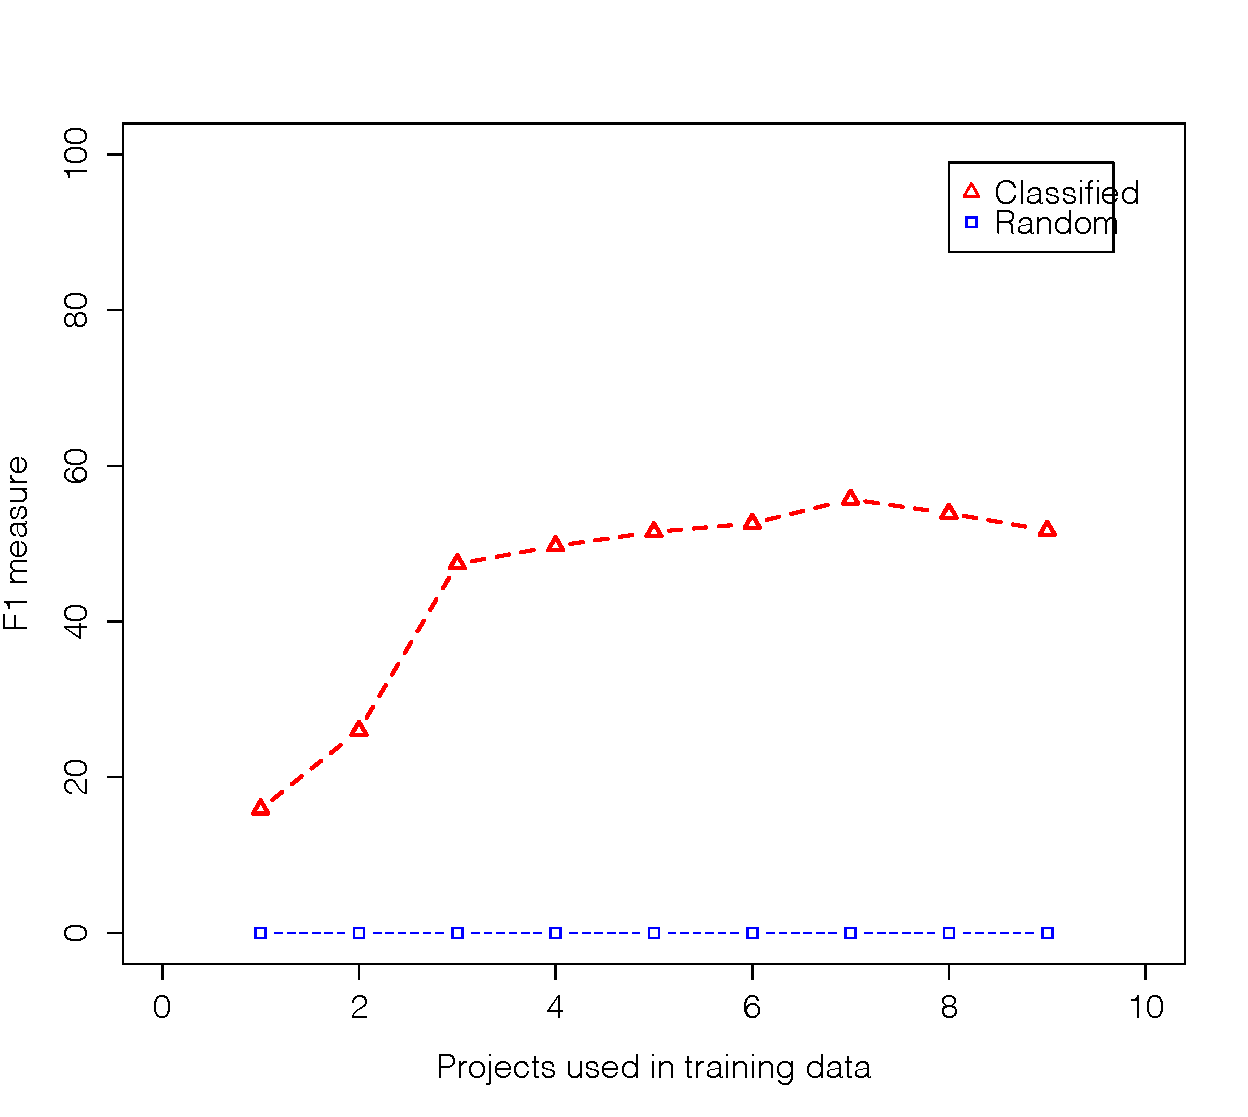
\includegraphics[width=0.50\textwidth]{figures/design_ant.pdf}
  \vspace{-3mm}
  \caption{Ant Design Debt classification}
  \label{fig:design_ant}
\end{figure}

\begin{figure}[thb!]
  \centering
  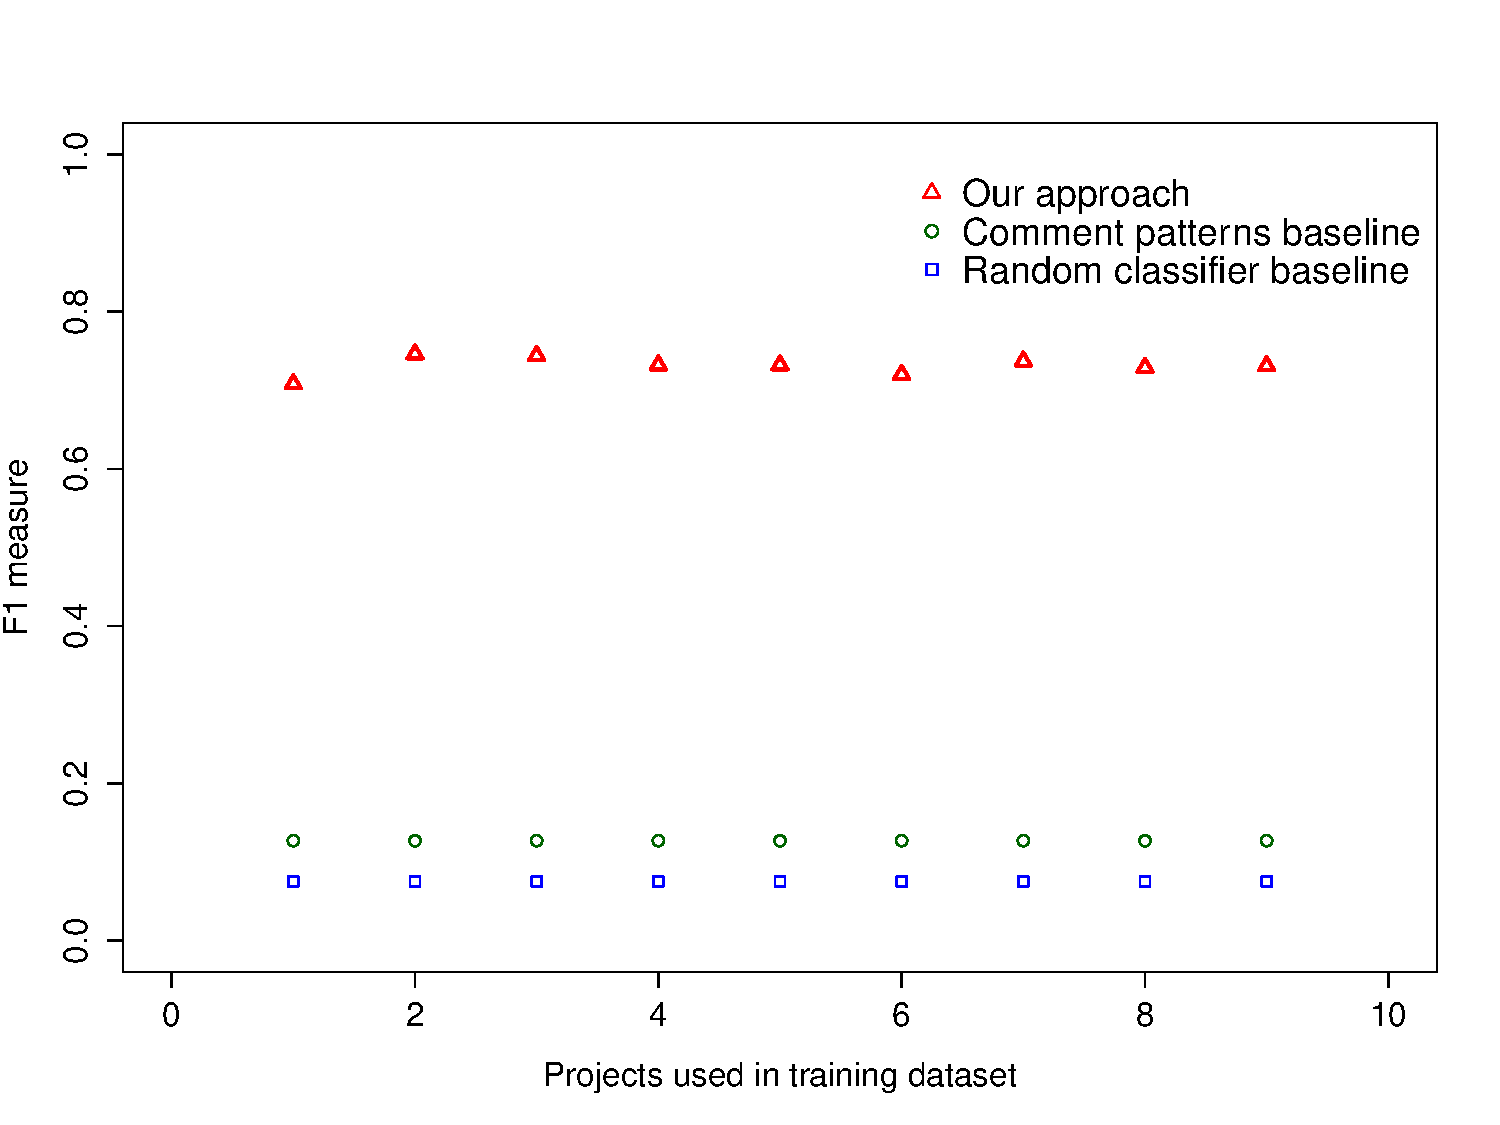
\includegraphics[width=0.50\textwidth]{figures/appendix/iteration_details/design_jmeter.pdf}
  \vspace{-3mm}
  \caption{Jmeter Design Debt classification}
  \label{fig:design_jmeter}
\end{figure}

\begin{figure}[thb!]
  \centering
  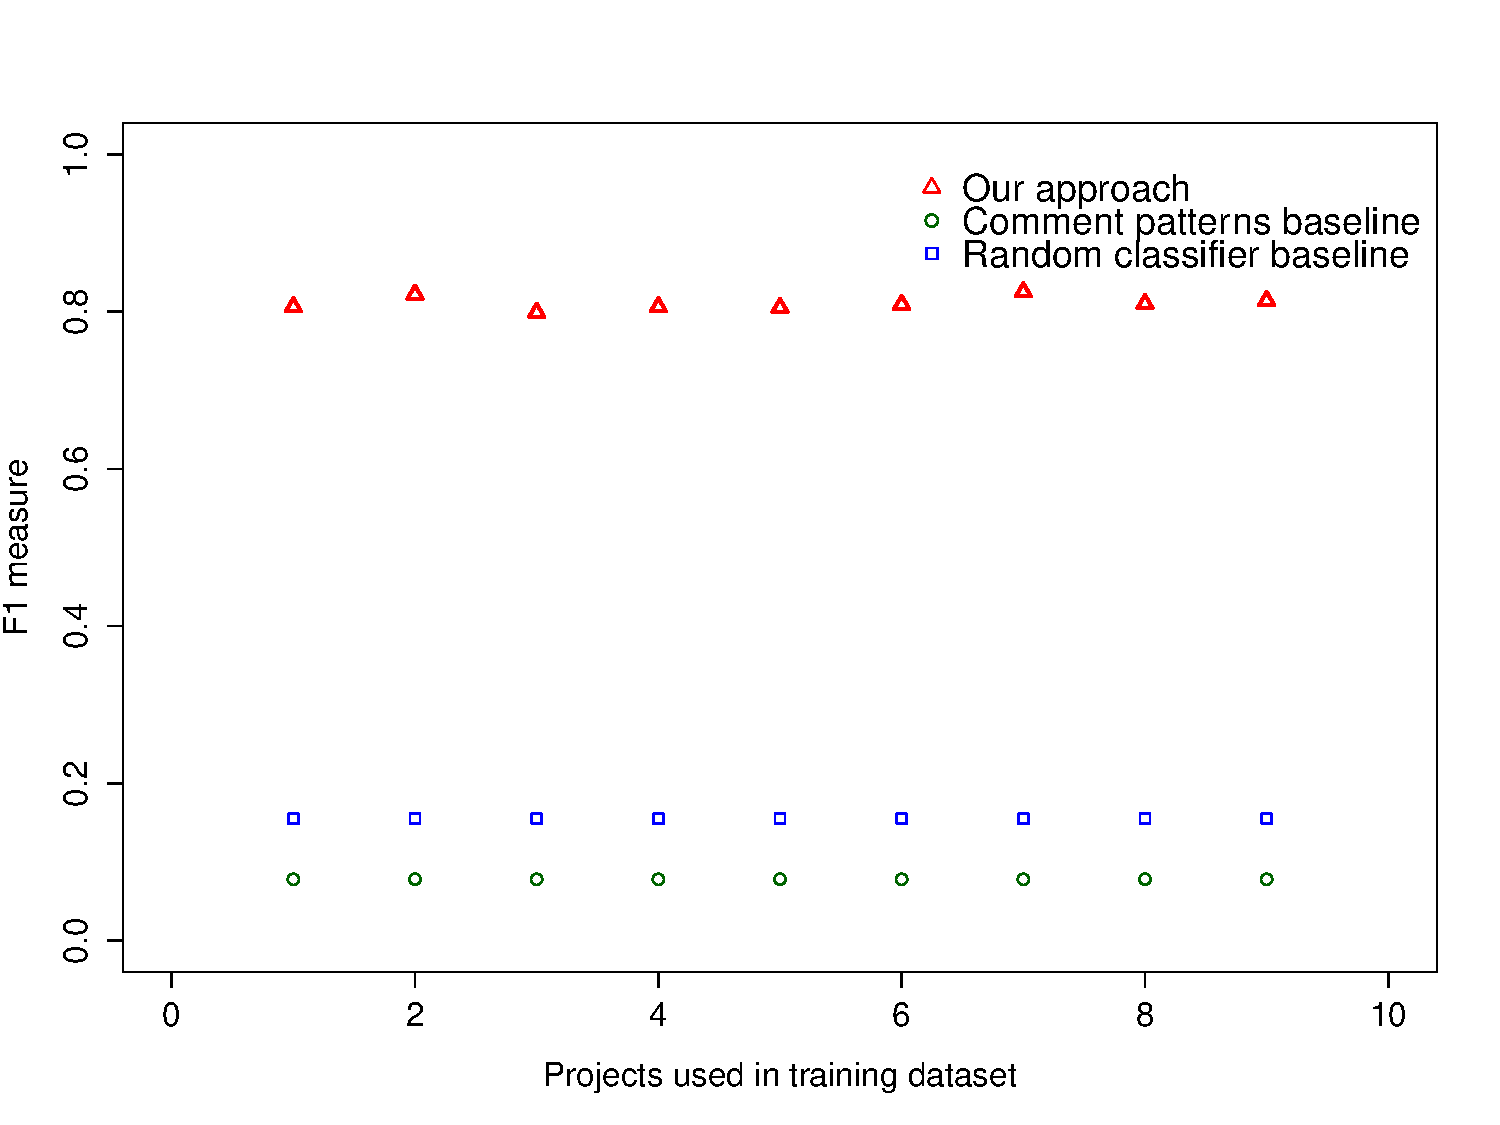
\includegraphics[width=0.50\textwidth]{figures/appendix/iteration_details/design_argo.pdf}
  \vspace{-3mm}
  \caption{Argo Design Debt classification}
  \label{fig:design_argo}
\end{figure}

\begin{figure}[thb!]
  \centering
  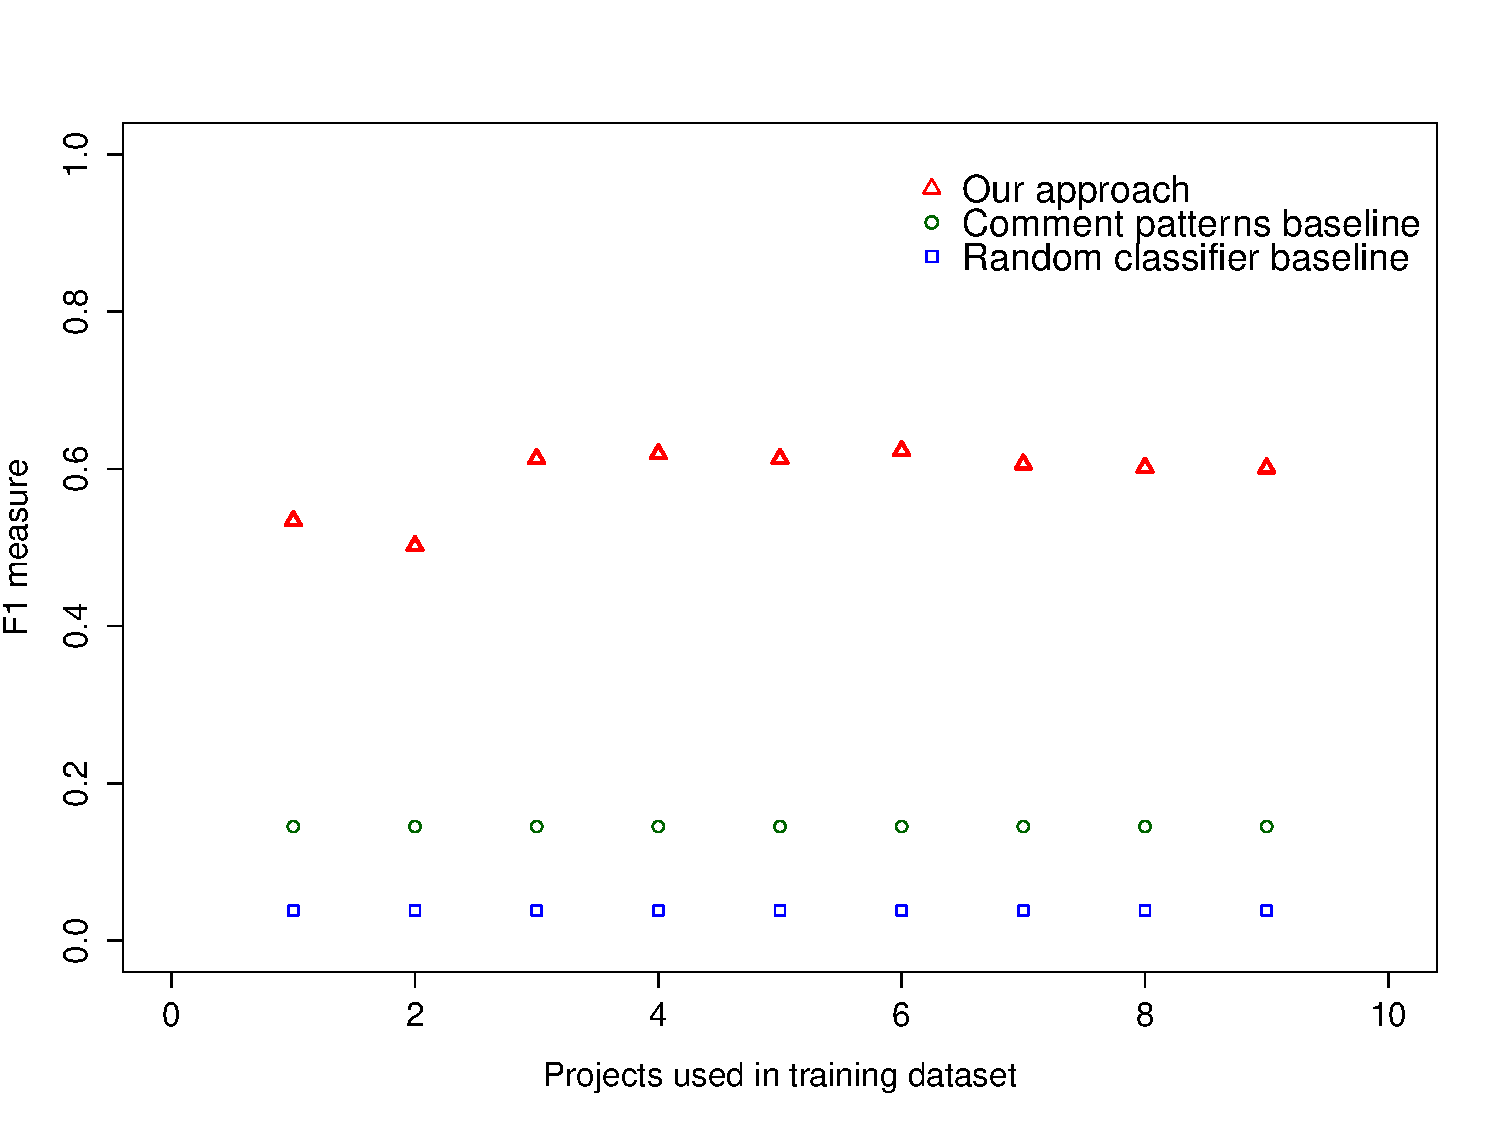
\includegraphics[width=0.50\textwidth]{figures/appendix/iteration_details/design_columba.pdf}
  \vspace{-3mm}
  \caption{Columba Design Debt classification}
  \label{fig:design_columba}
\end{figure}

\begin{figure}[thb!]
  \centering
  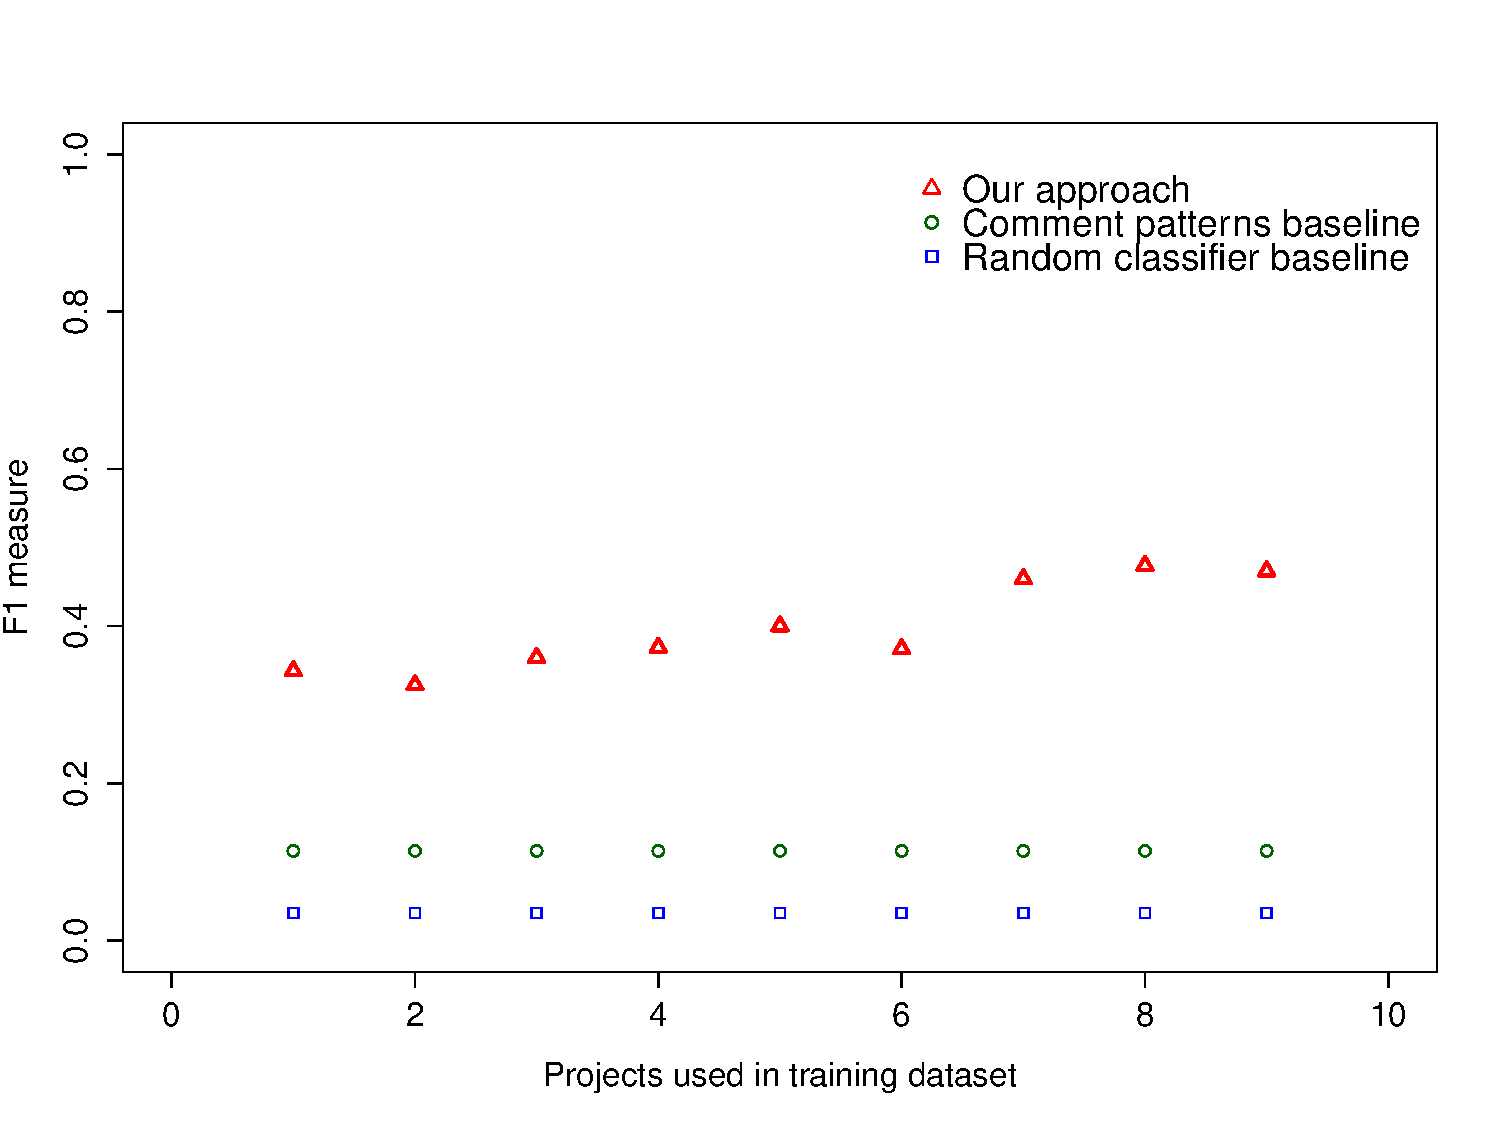
\includegraphics[width=0.50\textwidth]{figures/appendix/iteration_details/design_emf.pdf}
  \vspace{-3mm}
  \caption{Emf Design Debt classification}
  \label{fig:design_emf}
\end{figure}

\clearpage

\begin{figure}[thb!]
  \centering
  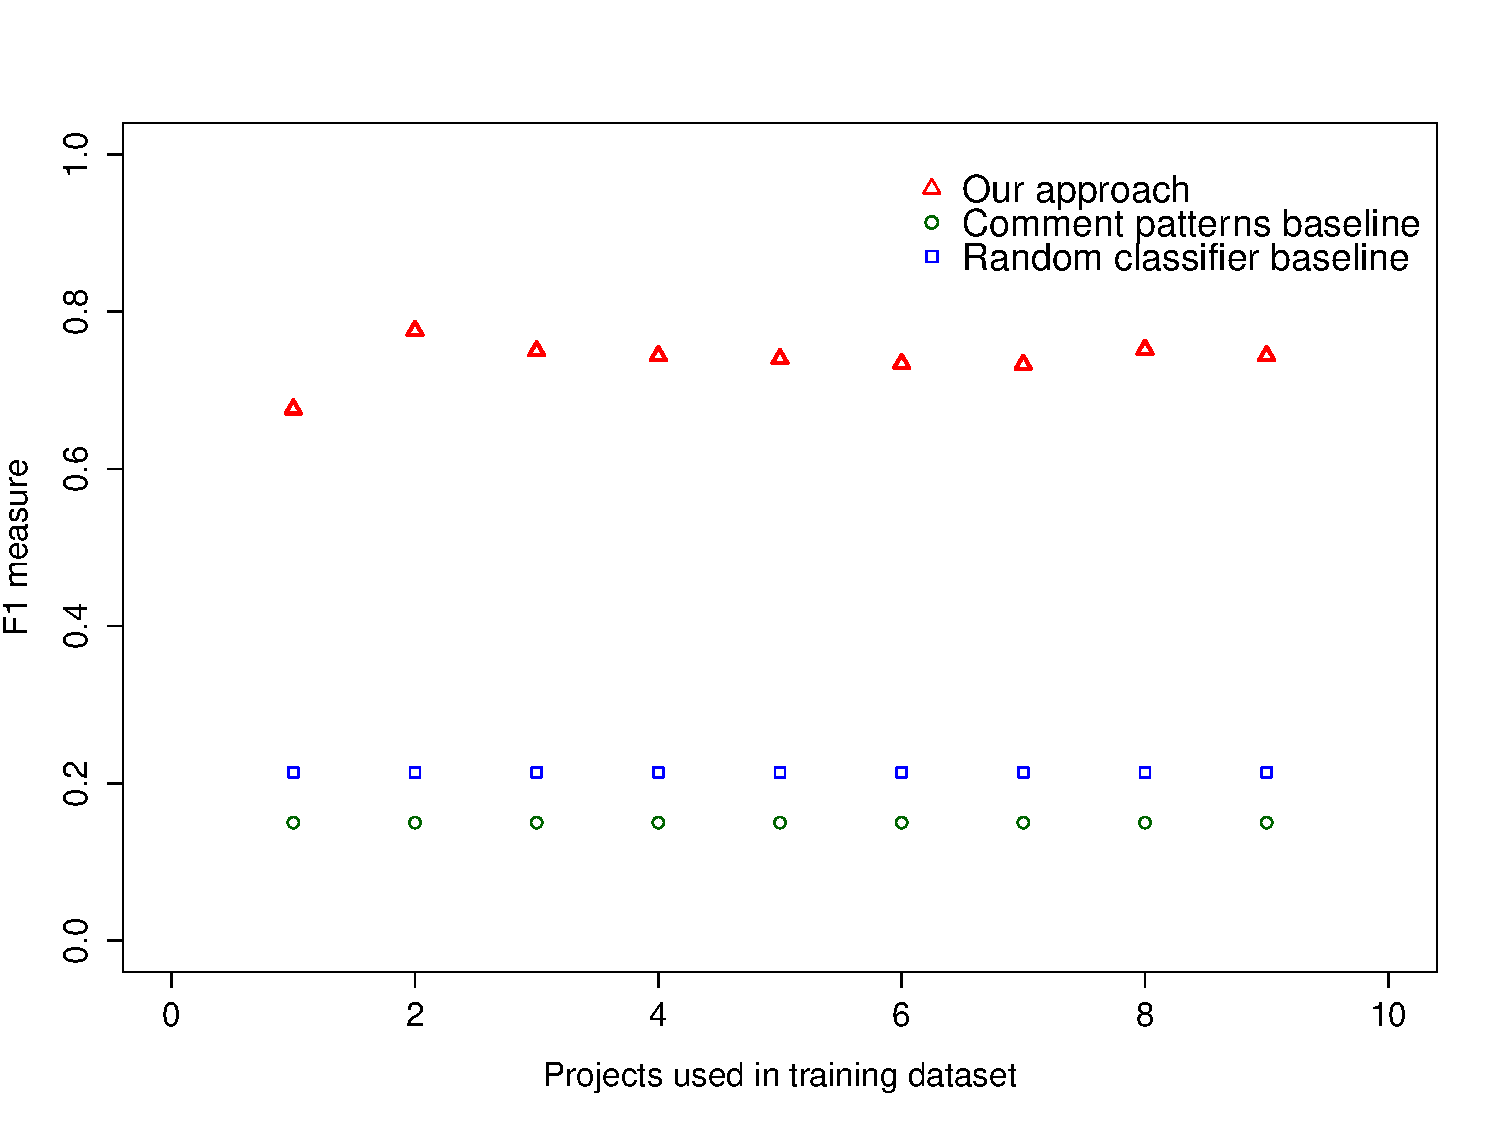
\includegraphics[width=0.50\textwidth]{figures/appendix/iteration_details/design_hibernate.pdf}
  \caption{Hibernate Design Debt classification}
  \label{fig:design_hibernate}
\end{figure}

\begin{figure}[thb!]
  \centering
  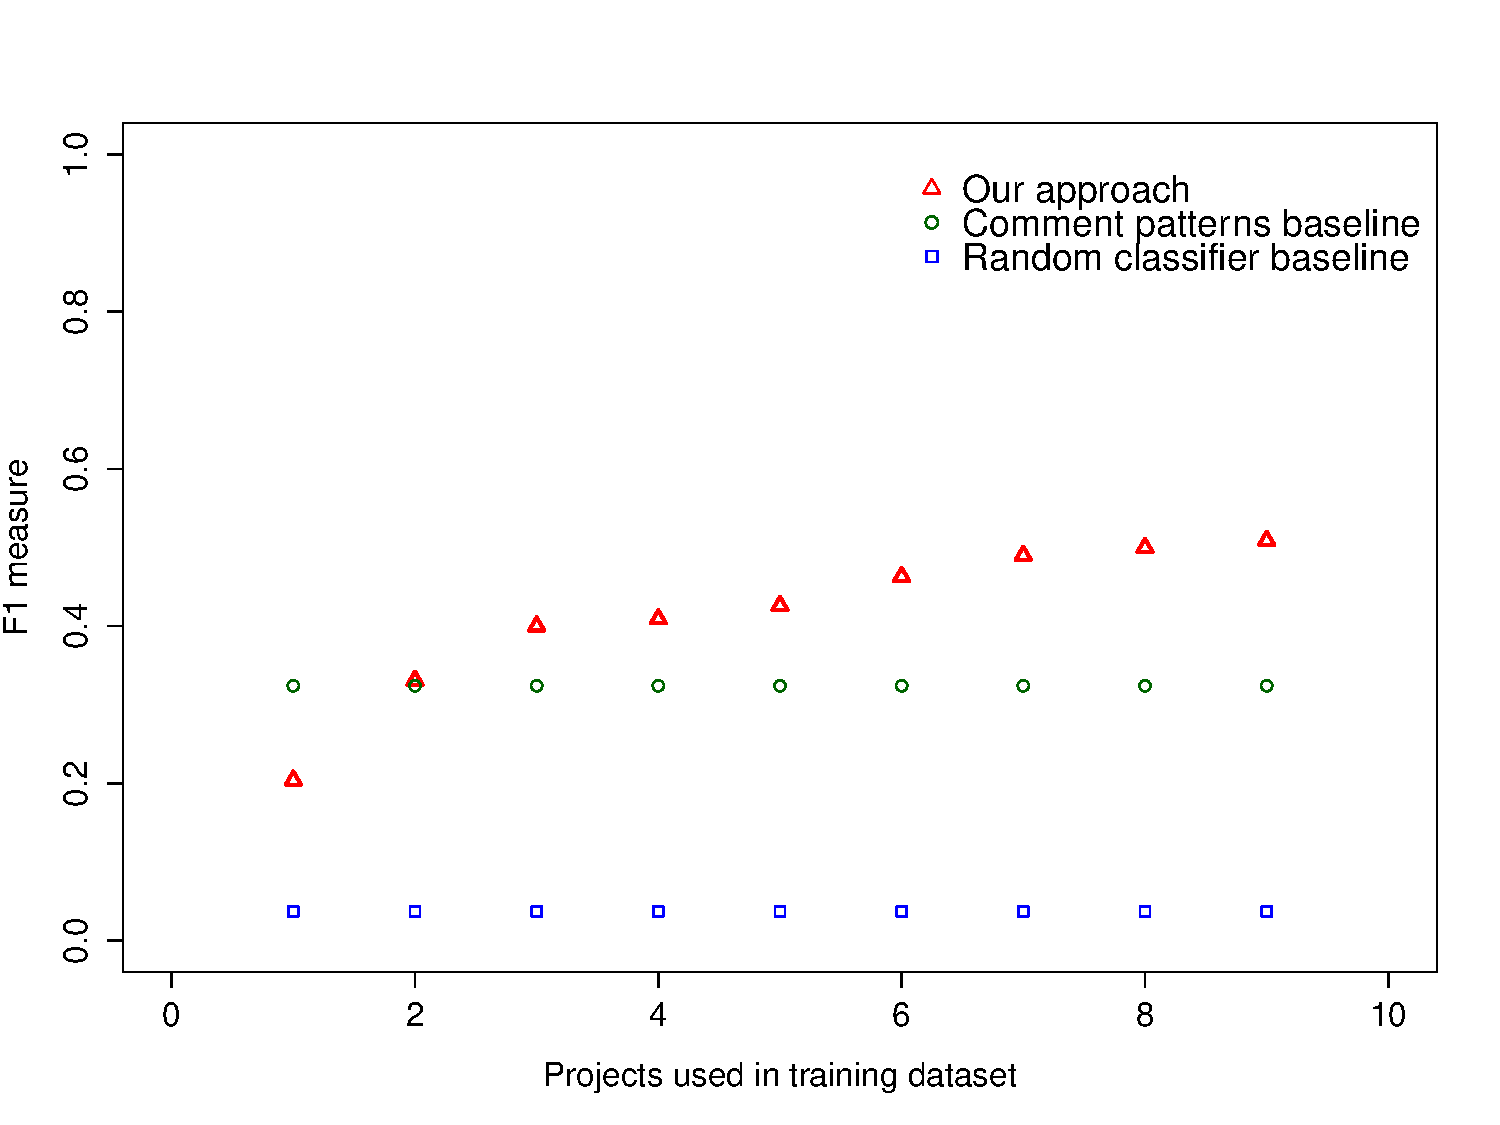
\includegraphics[width=0.50\textwidth]{figures/appendix/iteration_details/design_jedit.pdf}
  \vspace{-3mm}
  \caption{JEdit Design Debt classification}
  \label{fig:design_jedit}
\end{figure}

\begin{figure}[thb!]
  \centering
  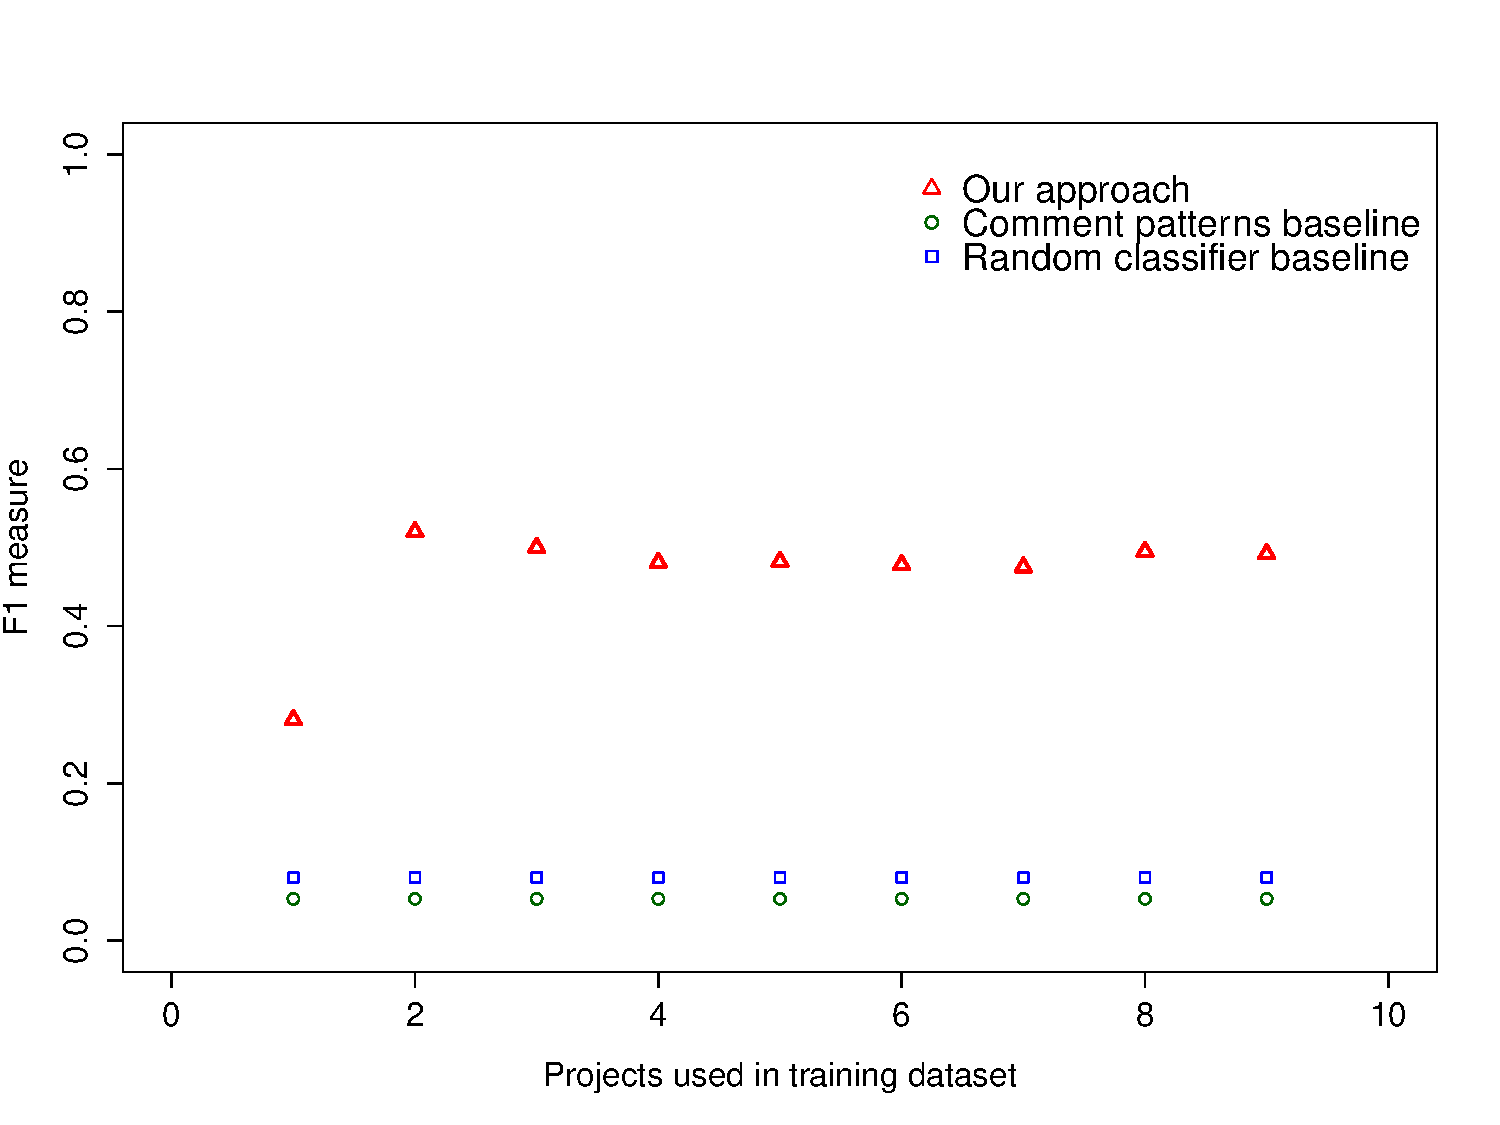
\includegraphics[width=0.50\textwidth]{figures/appendix/iteration_details/design_jfreechart.pdf}
  \vspace{-3mm}
  \caption{JFreeChart Design Debt classification}
  \label{fig:design_jfreechart}
\end{figure}

\begin{figure}[thb!]
  \centering
  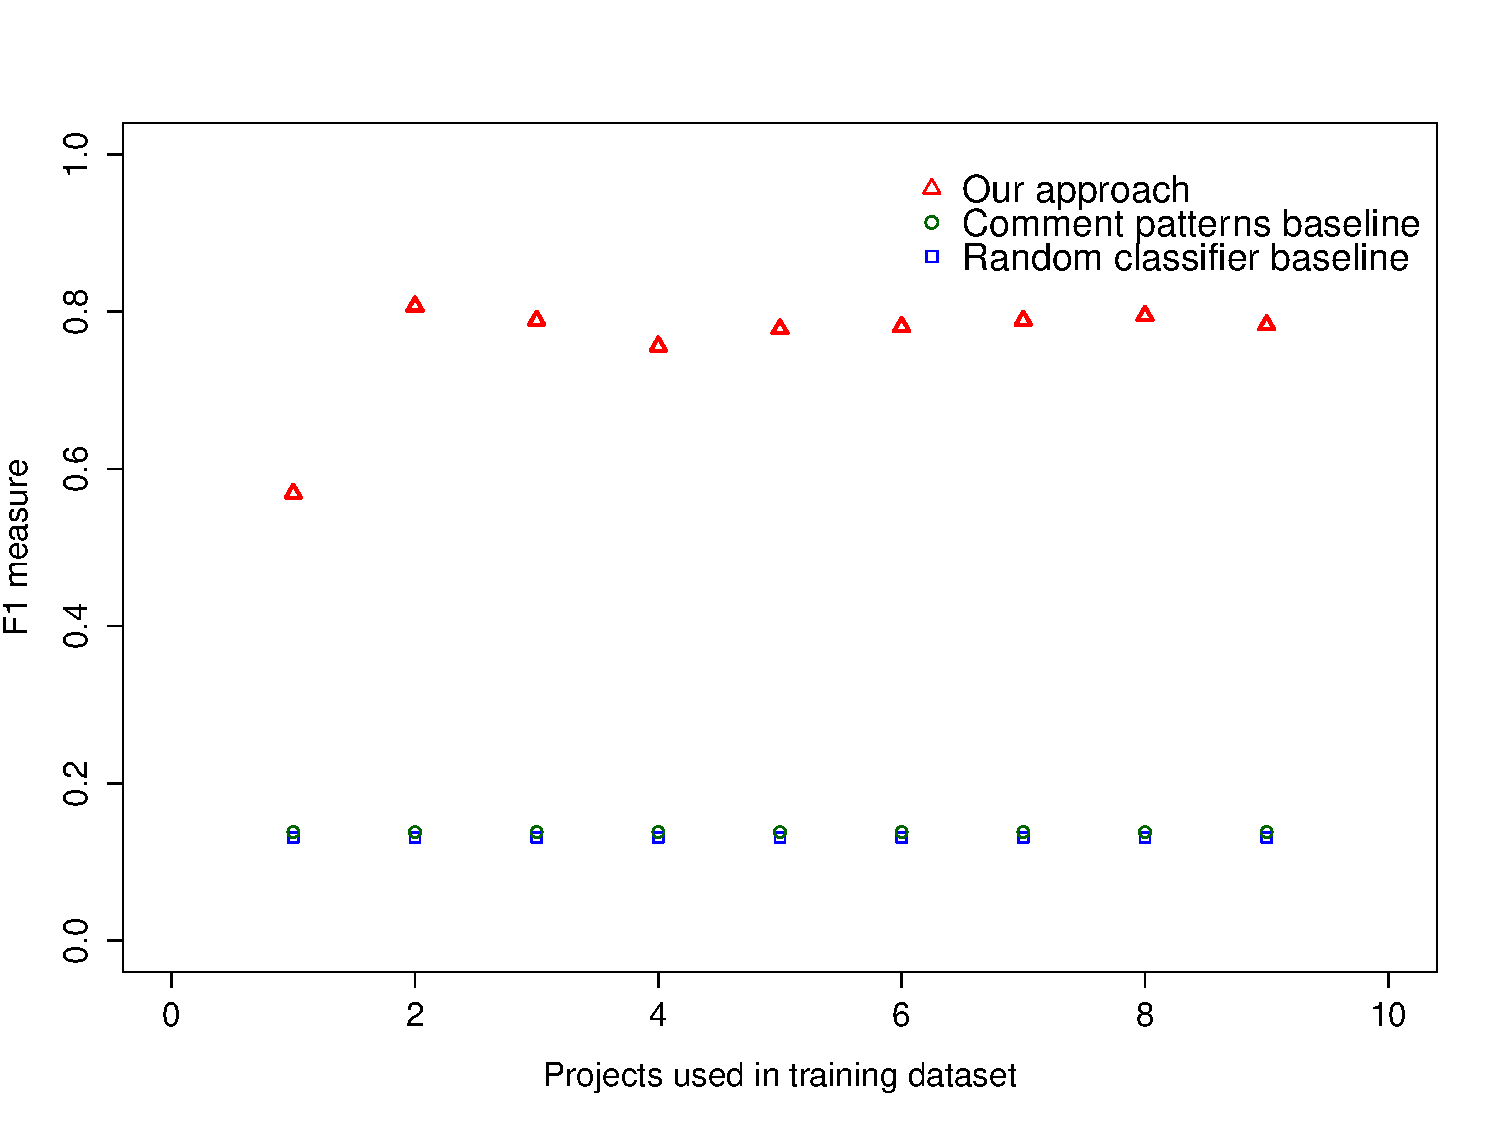
\includegraphics[width=0.50\textwidth]{figures/appendix/iteration_details/design_jruby.pdf}
  \vspace{-3mm}
  \caption{JRuby Design Debt classification}
  \label{fig:design_jruby}
\end{figure}

\begin{figure}[thb!]
  \centering
  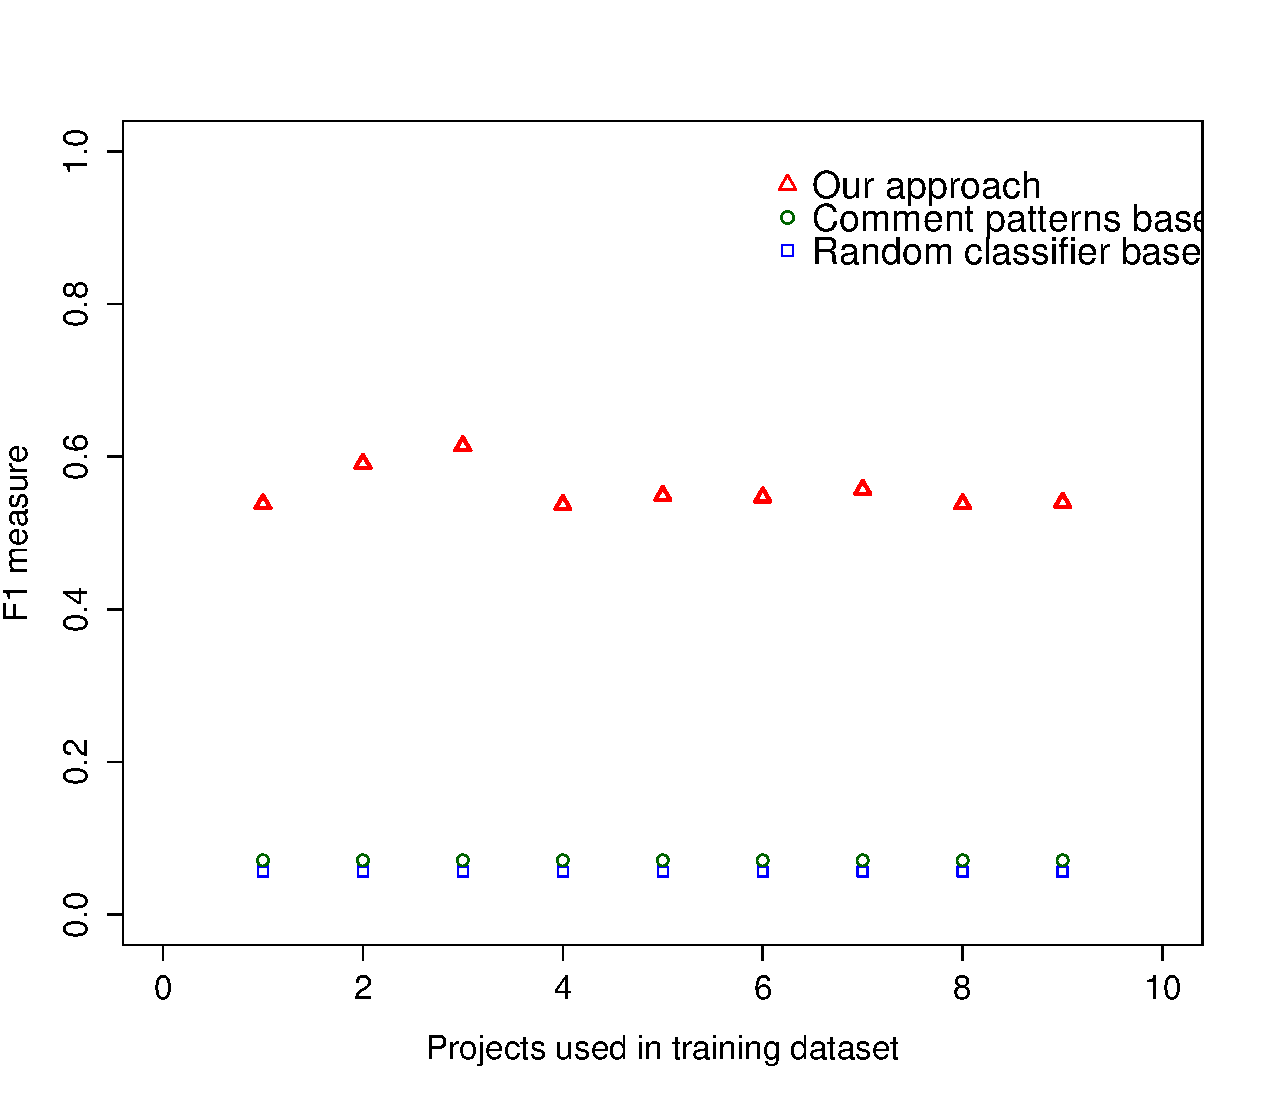
\includegraphics[width=0.50\textwidth]{figures/appendix/iteration_details/design_sql12.pdf}
  \vspace{-3mm}
  \caption{SQuirrel Design Debt classification}
  \label{fig:design_sql}
\end{figure}

\clearpage
 
\begin{figure}[thb!]    
  \centering
  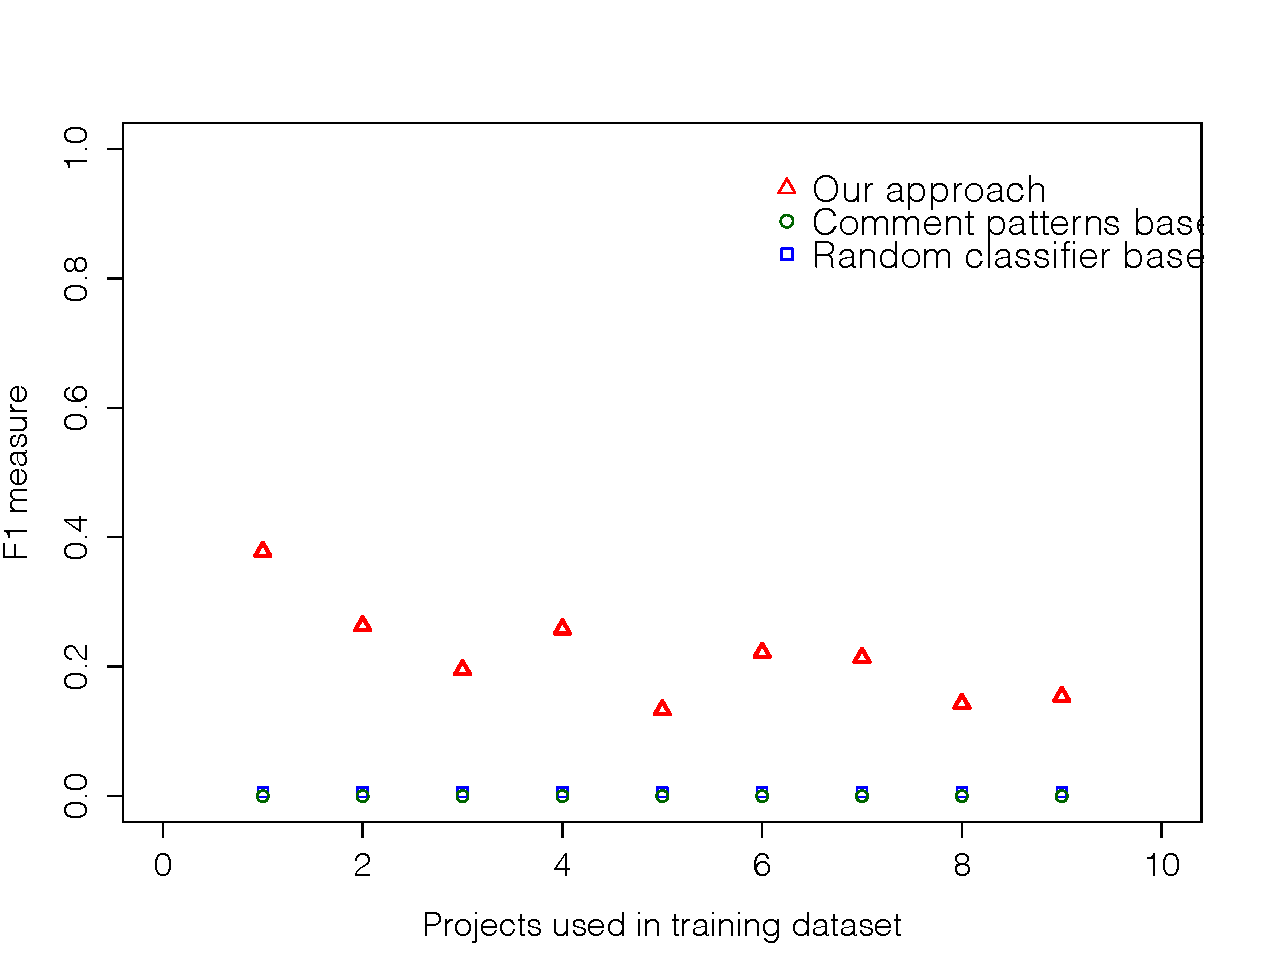
\includegraphics[width=0.50\textwidth]{figures/appendix/iteration_details/implementation_ant.pdf}
  \vspace{-3mm}
  \caption{Ant Requirement Debt classification}
  \label{fig:implementation_ant}
\end{figure}

\begin{figure}[thb!]
  \centering
  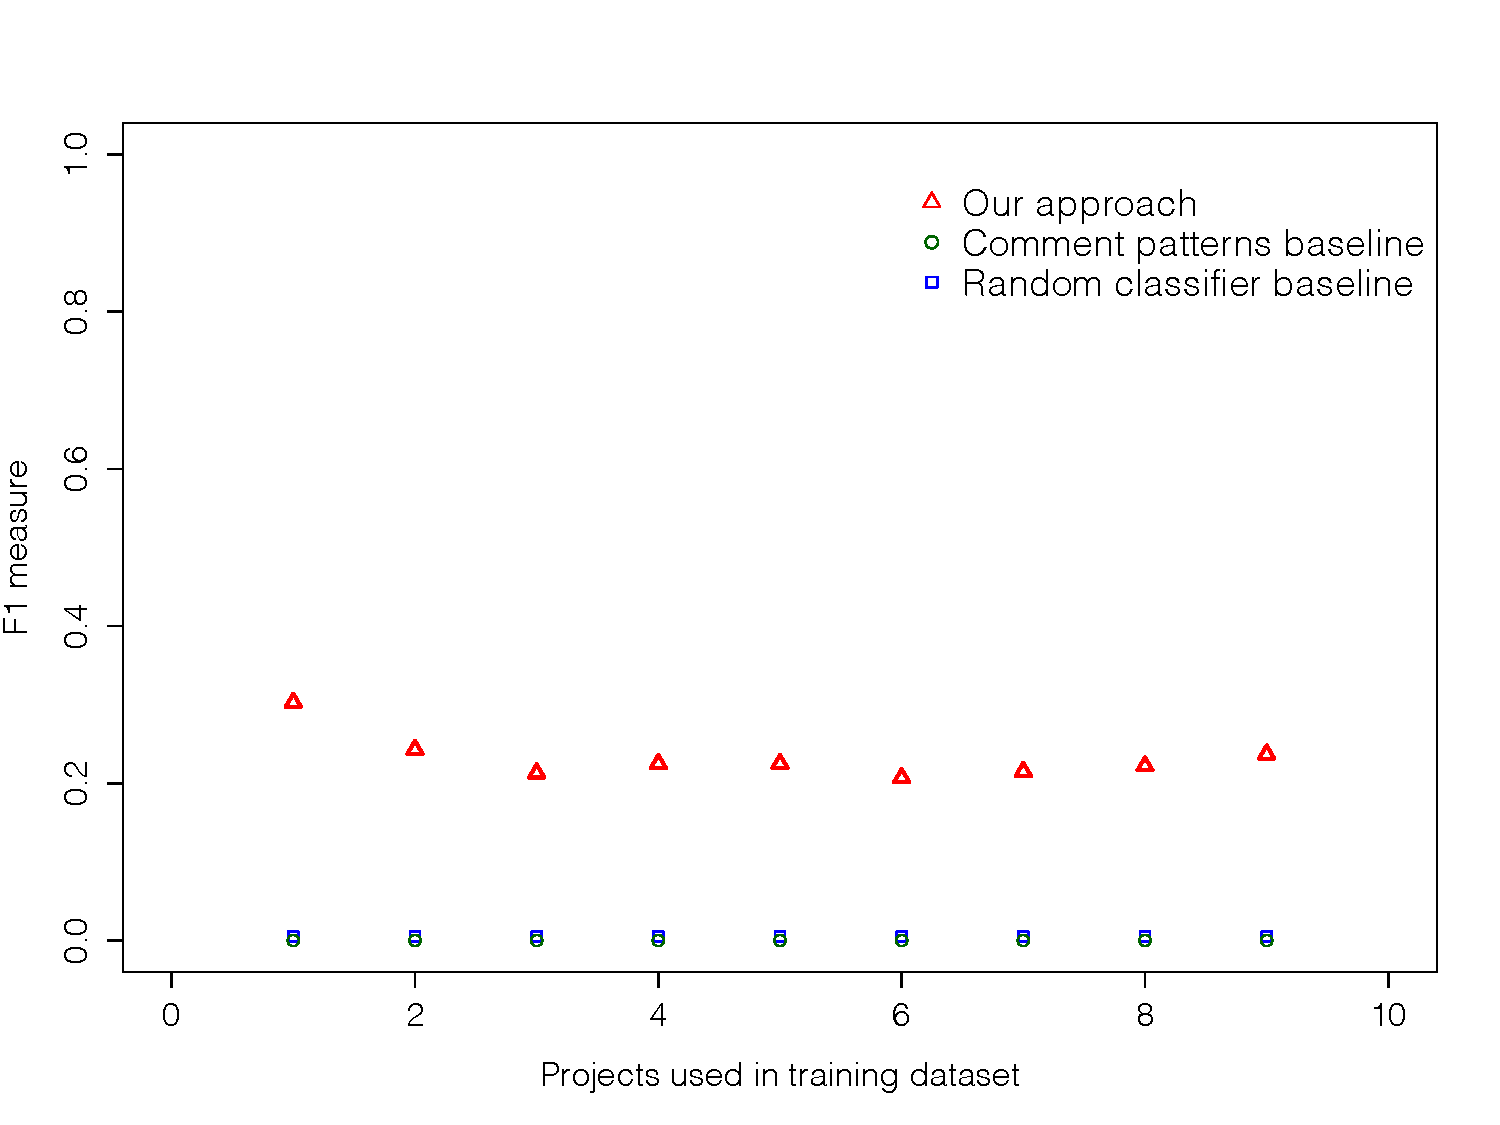
\includegraphics[width=0.50\textwidth]{figures/appendix/iteration_details/implementation_jmeter.pdf}
  \vspace{-3mm}
  \caption{Jmeter Requirement Debt classification}
  \label{fig:implementation_jmeter}
\end{figure}

\begin{figure}[thb!]
  \centering
  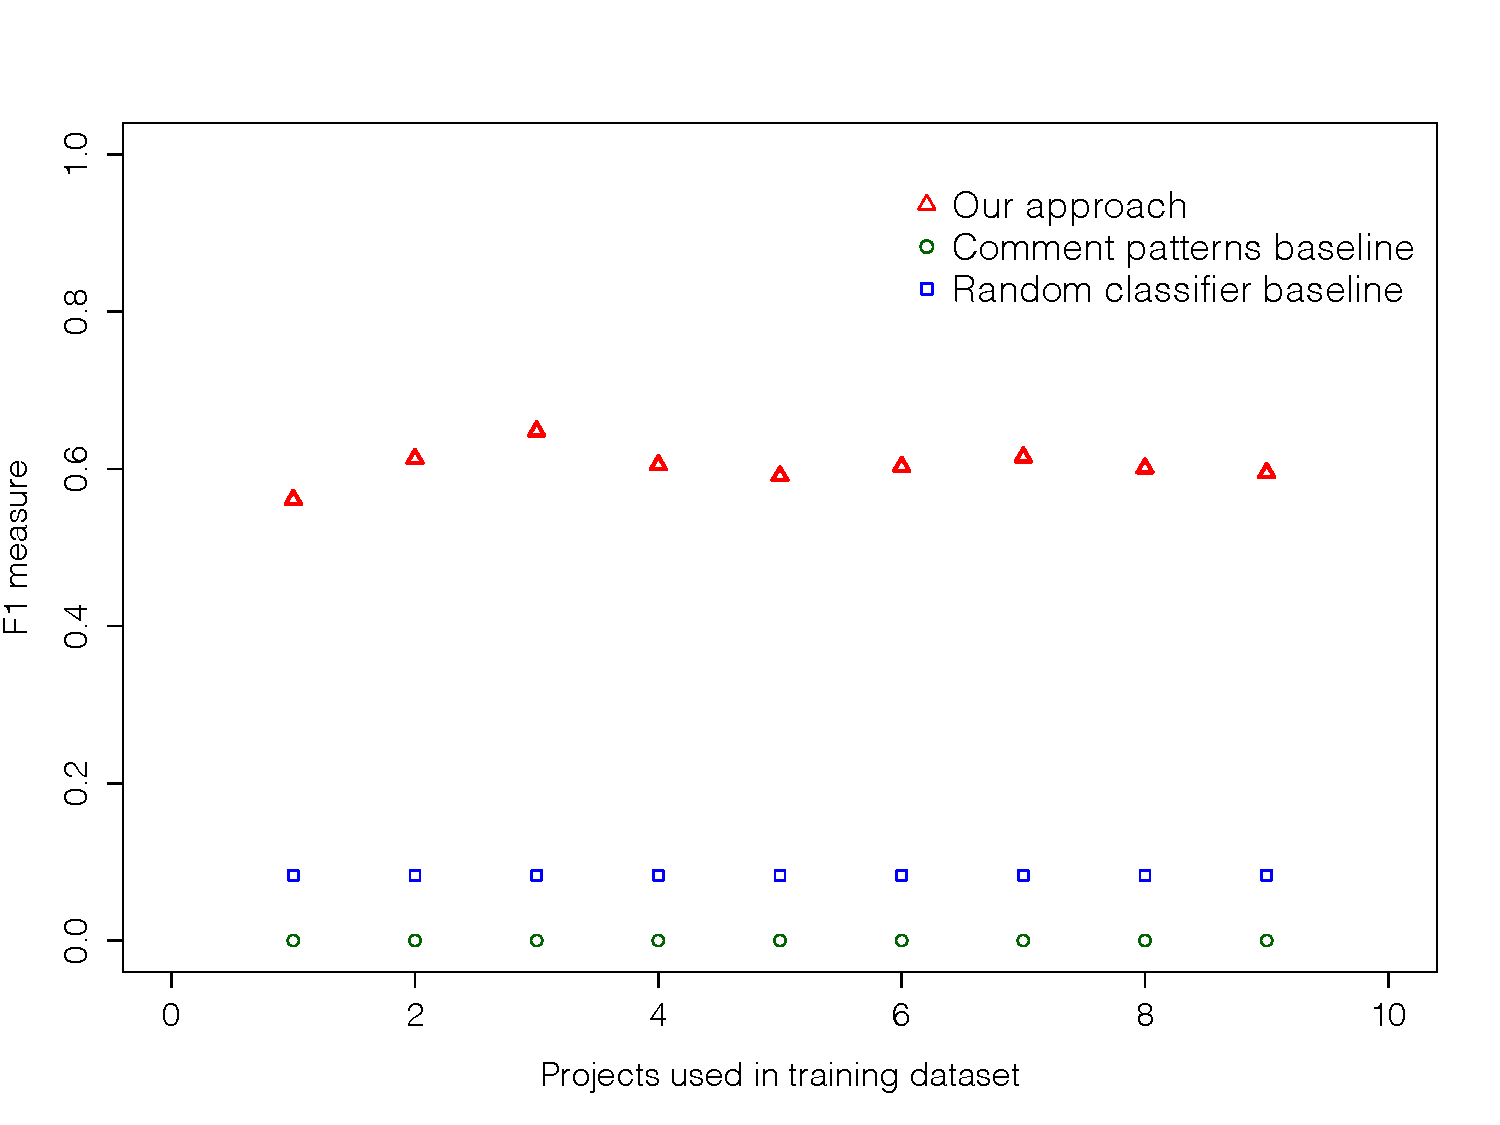
\includegraphics[width=0.50\textwidth]{figures/appendix/iteration_details/implementation_argo.pdf}
  \vspace{-3mm}
  \caption{Argo Requirement Debt classification}
  \label{fig:implementation_argo}
\end{figure}

\begin{figure}[thb!]
  \centering
  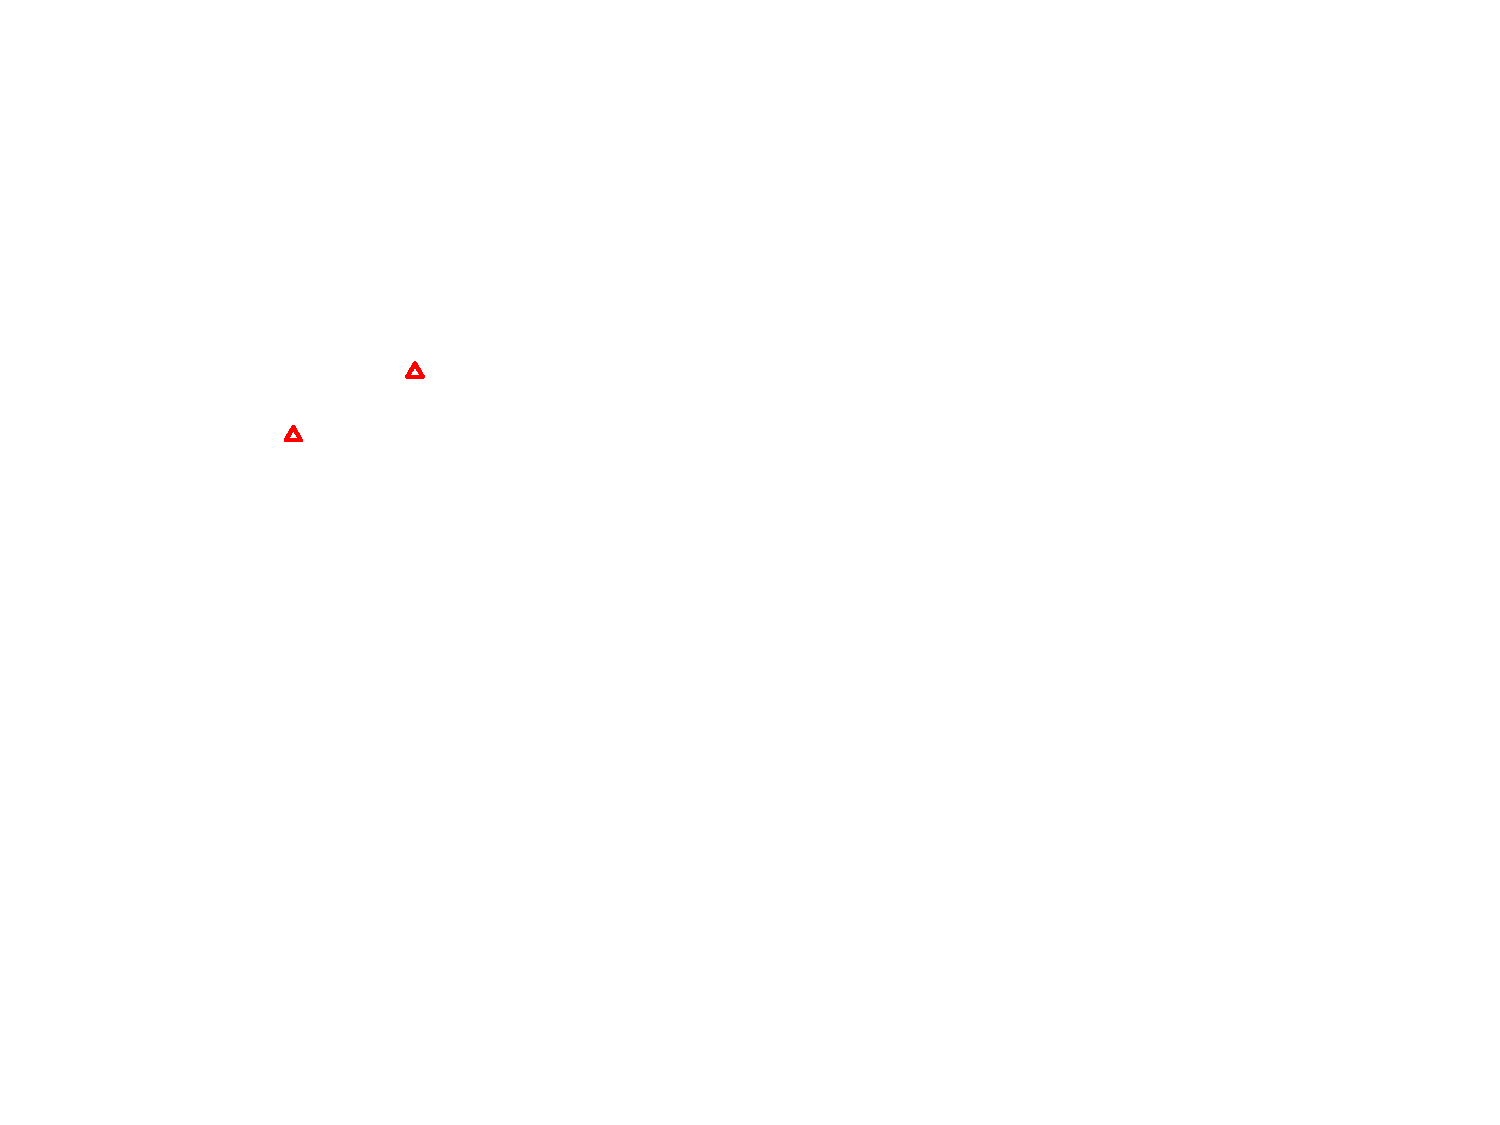
\includegraphics[width=0.50\textwidth]{figures/appendix/iteration_details/implementation_columba.pdf}
  \vspace{-3mm}
  \caption{Columba Requirement Debt classification}
  \label{fig:implementation_columba}
\end{figure}

\begin{figure}[thb!]
  \centering
  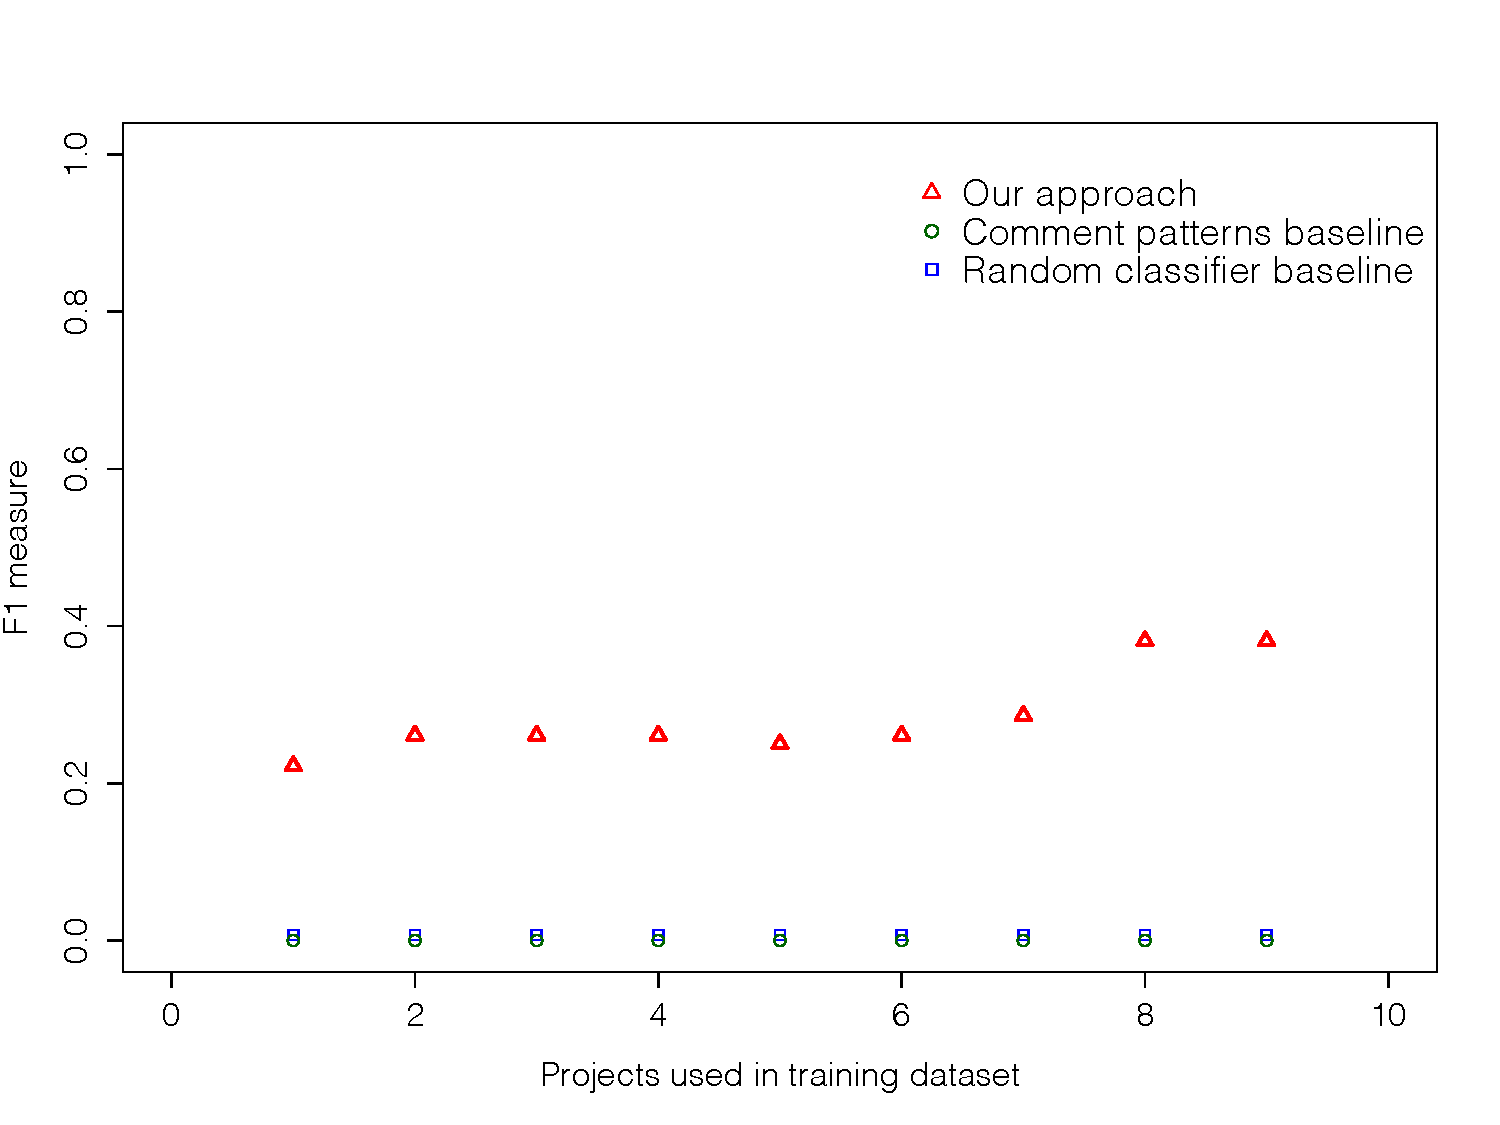
\includegraphics[width=0.50\textwidth]{figures/appendix/iteration_details/implementation_emf.pdf}
  \vspace{-3mm}
  \caption{Emf Requirement Debt classification}
  \label{fig:implementation_emf}
\end{figure}

\clearpage

\begin{figure}[thb!]
  \centering
  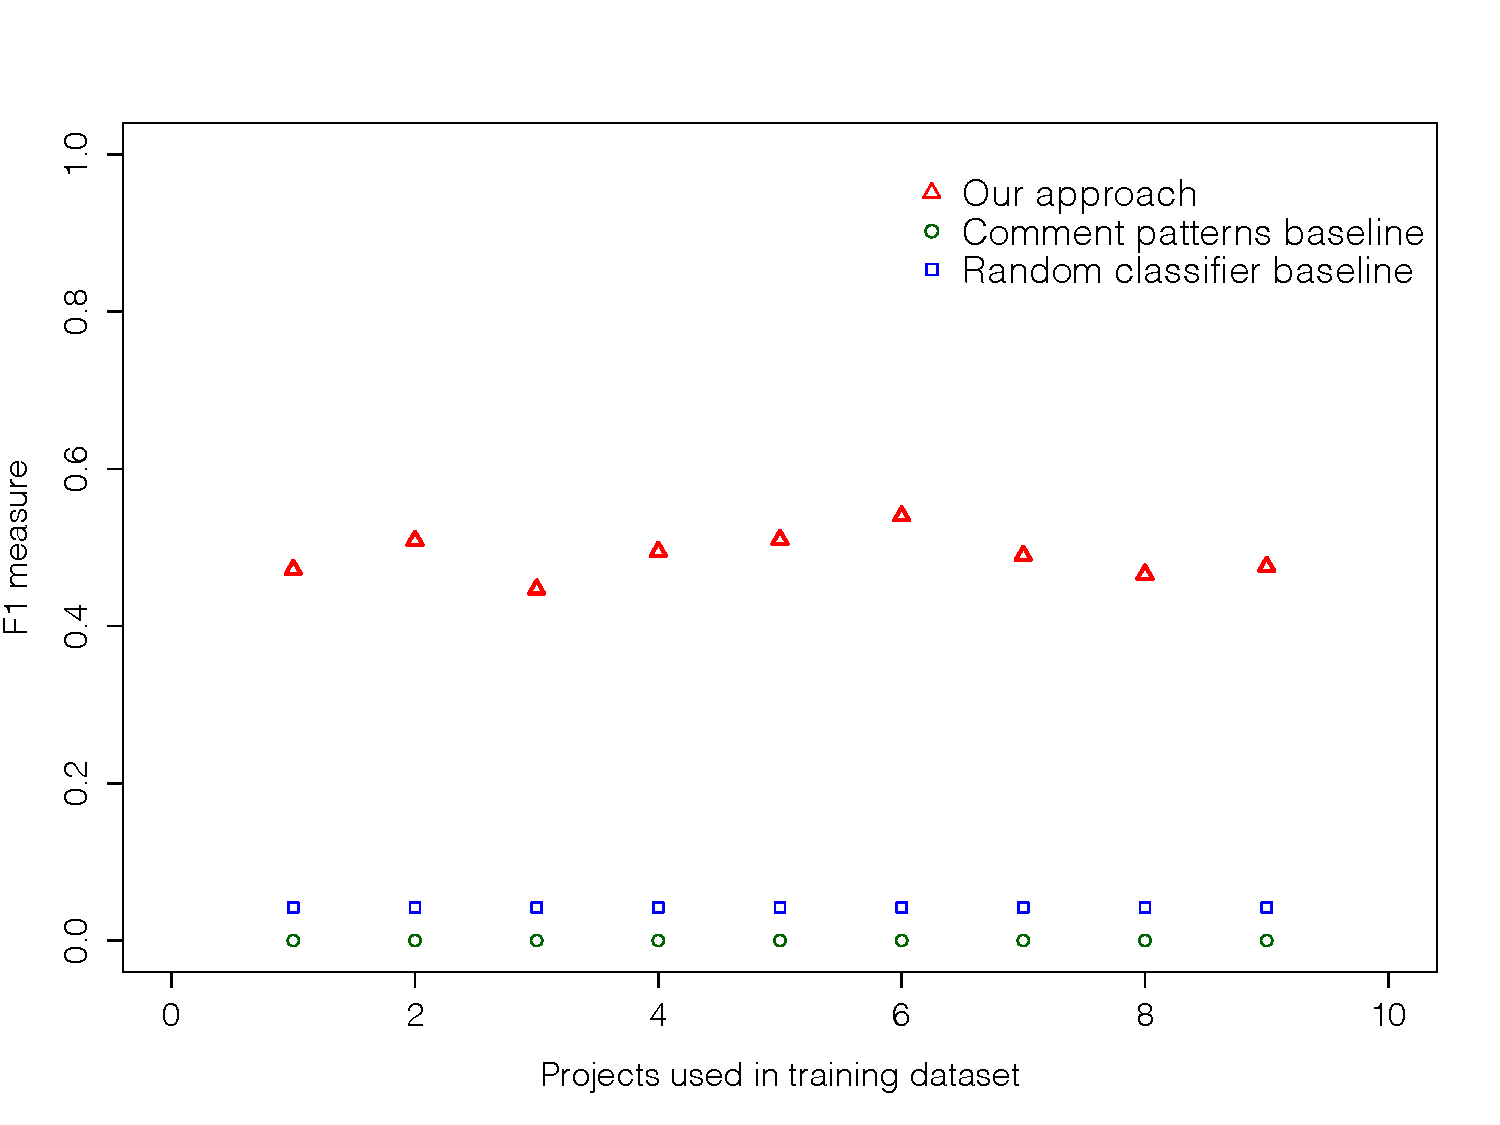
\includegraphics[width=0.50\textwidth]{figures/appendix/iteration_details/implementation_hibernate.pdf}
  \caption{Hibernate Requirement Debt classification}
  \label{fig:implementation_hibernate}
\end{figure}

\begin{figure}[thb!]
  \centering
  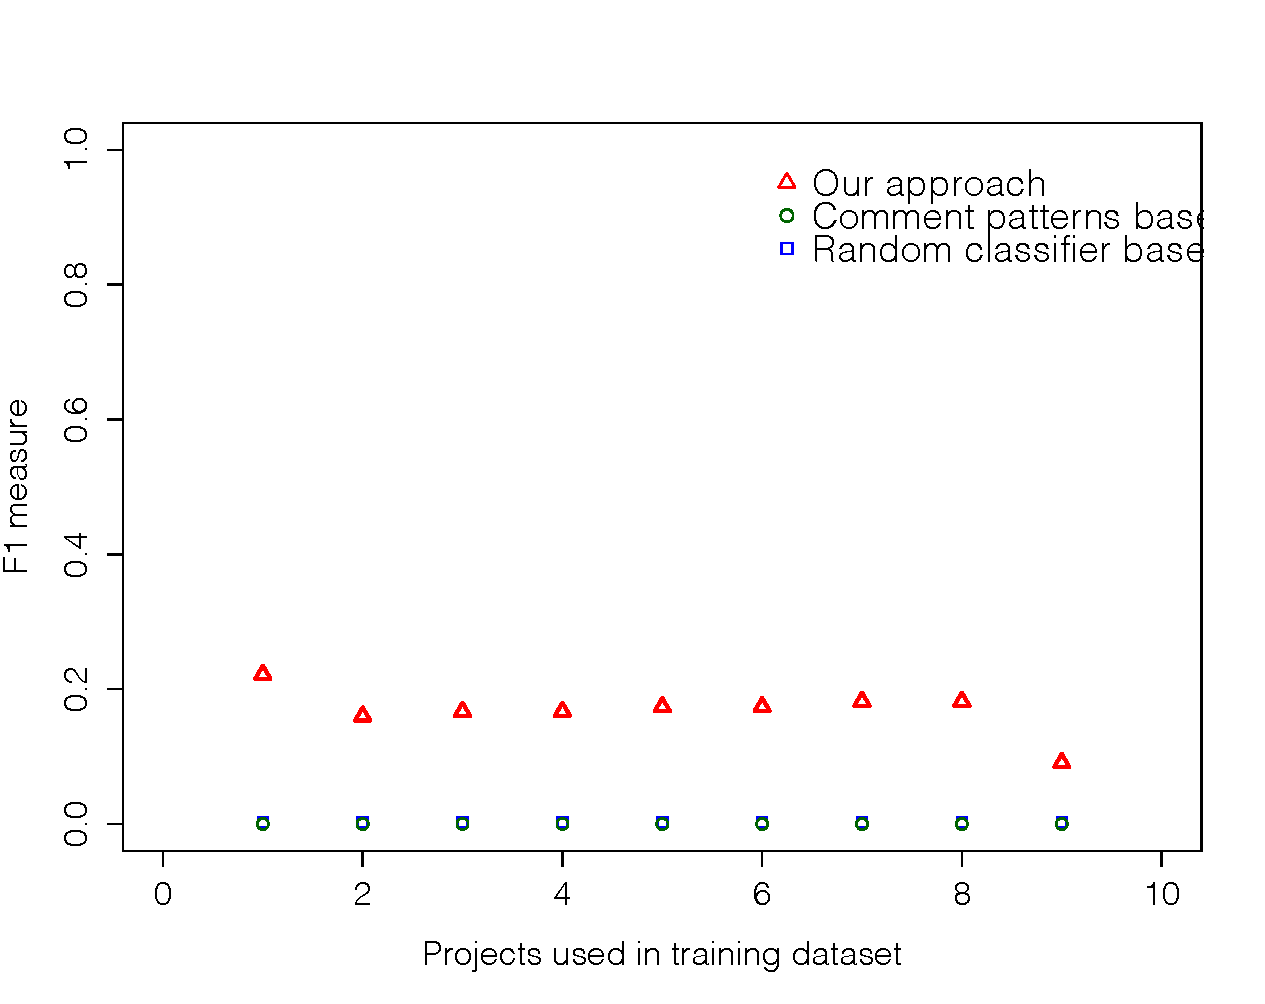
\includegraphics[width=0.50\textwidth]{figures/appendix/iteration_details/implementation_jedit.pdf}
  \vspace{-3mm}
  \caption{JEdit Requirement Debt classification}
  \label{fig:implementation_jedit}
\end{figure}

\begin{figure}[thb!]
  \centering
  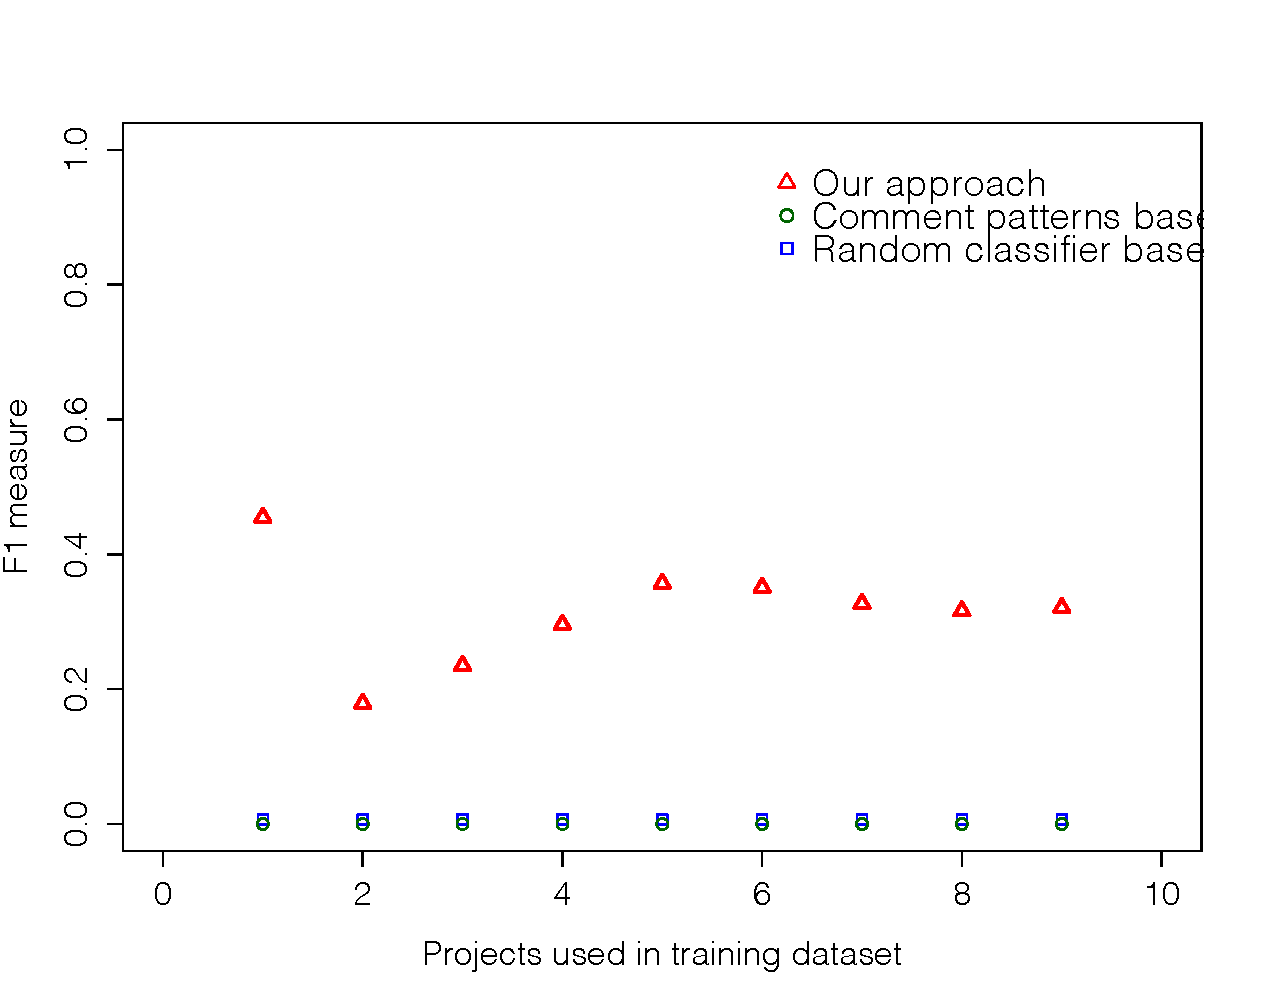
\includegraphics[width=0.50\textwidth]{figures/appendix/iteration_details/implementation_jfreechart.pdf}
  \vspace{-3mm}
  \caption{JFreeChart Requirement Debt classification}
  \label{fig:implementation_jfreechart}
\end{figure}

\begin{figure}[thb!]
  \centering
  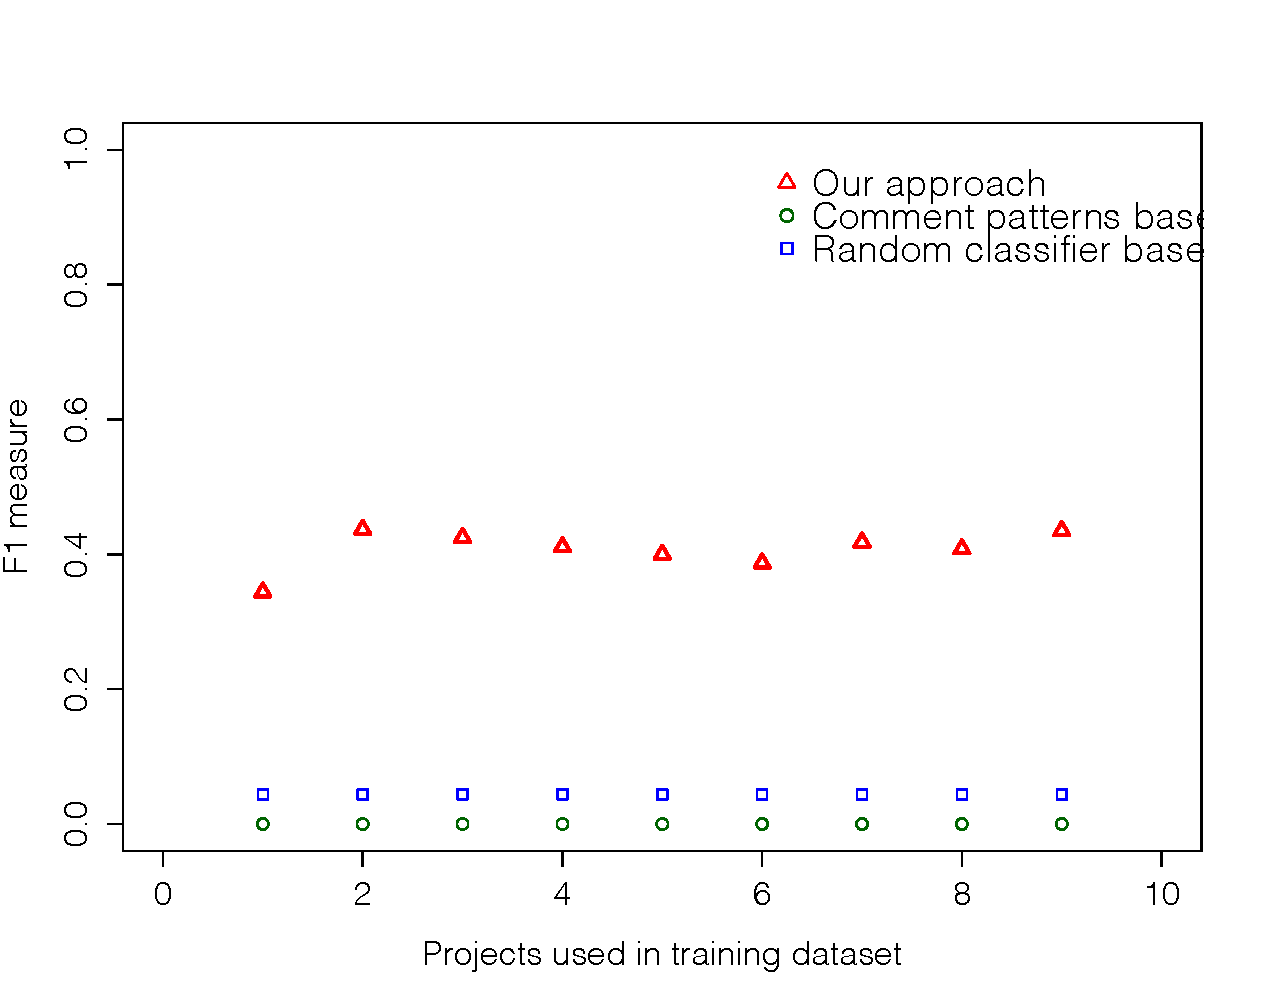
\includegraphics[width=0.50\textwidth]{figures/appendix/iteration_details/implementation_jruby.pdf}
  \vspace{-3mm}
  \caption{JRuby Requirement Debt classification}
  \label{fig:implementation_jruby}
\end{figure}

\begin{figure}[thb!]
  \centering
  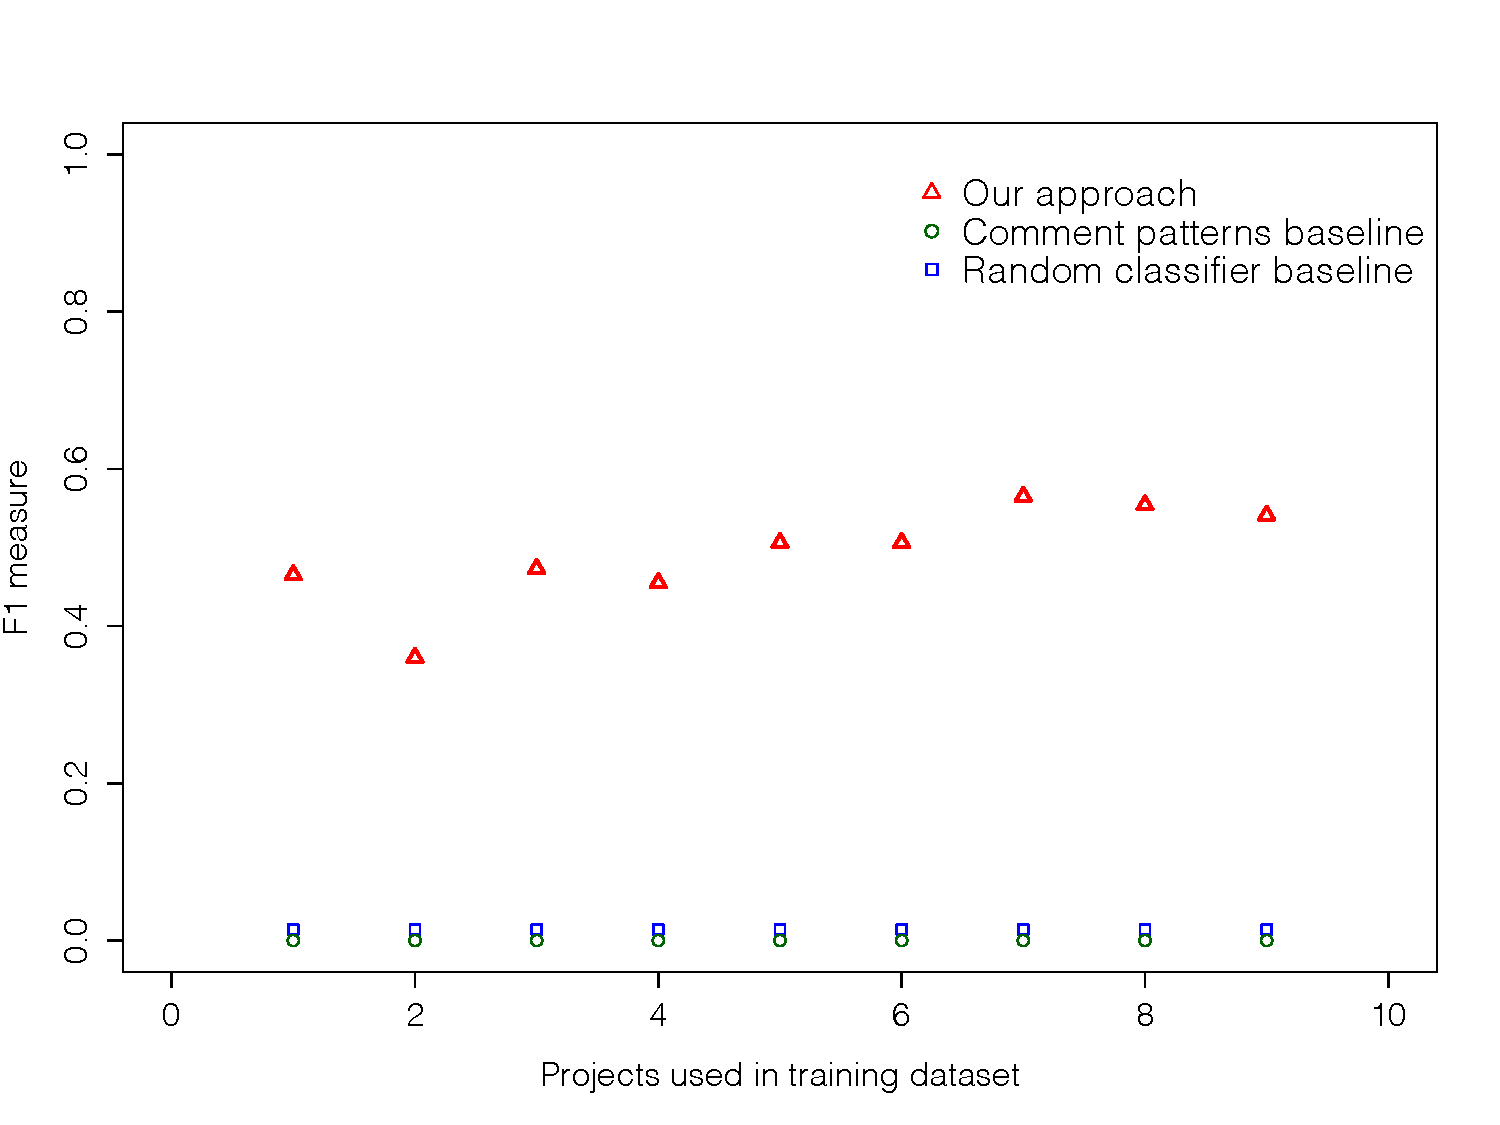
\includegraphics[width=0.50\textwidth]{figures/appendix/iteration_details/implementation_sql12.pdf}
  \vspace{-3mm}
  \caption{SQuirrel Requirement Debt classification}
  \label{fig:implementation_sql}
\end{figure}

\clearpage

\begin{figure}[thb!]
  \centering
  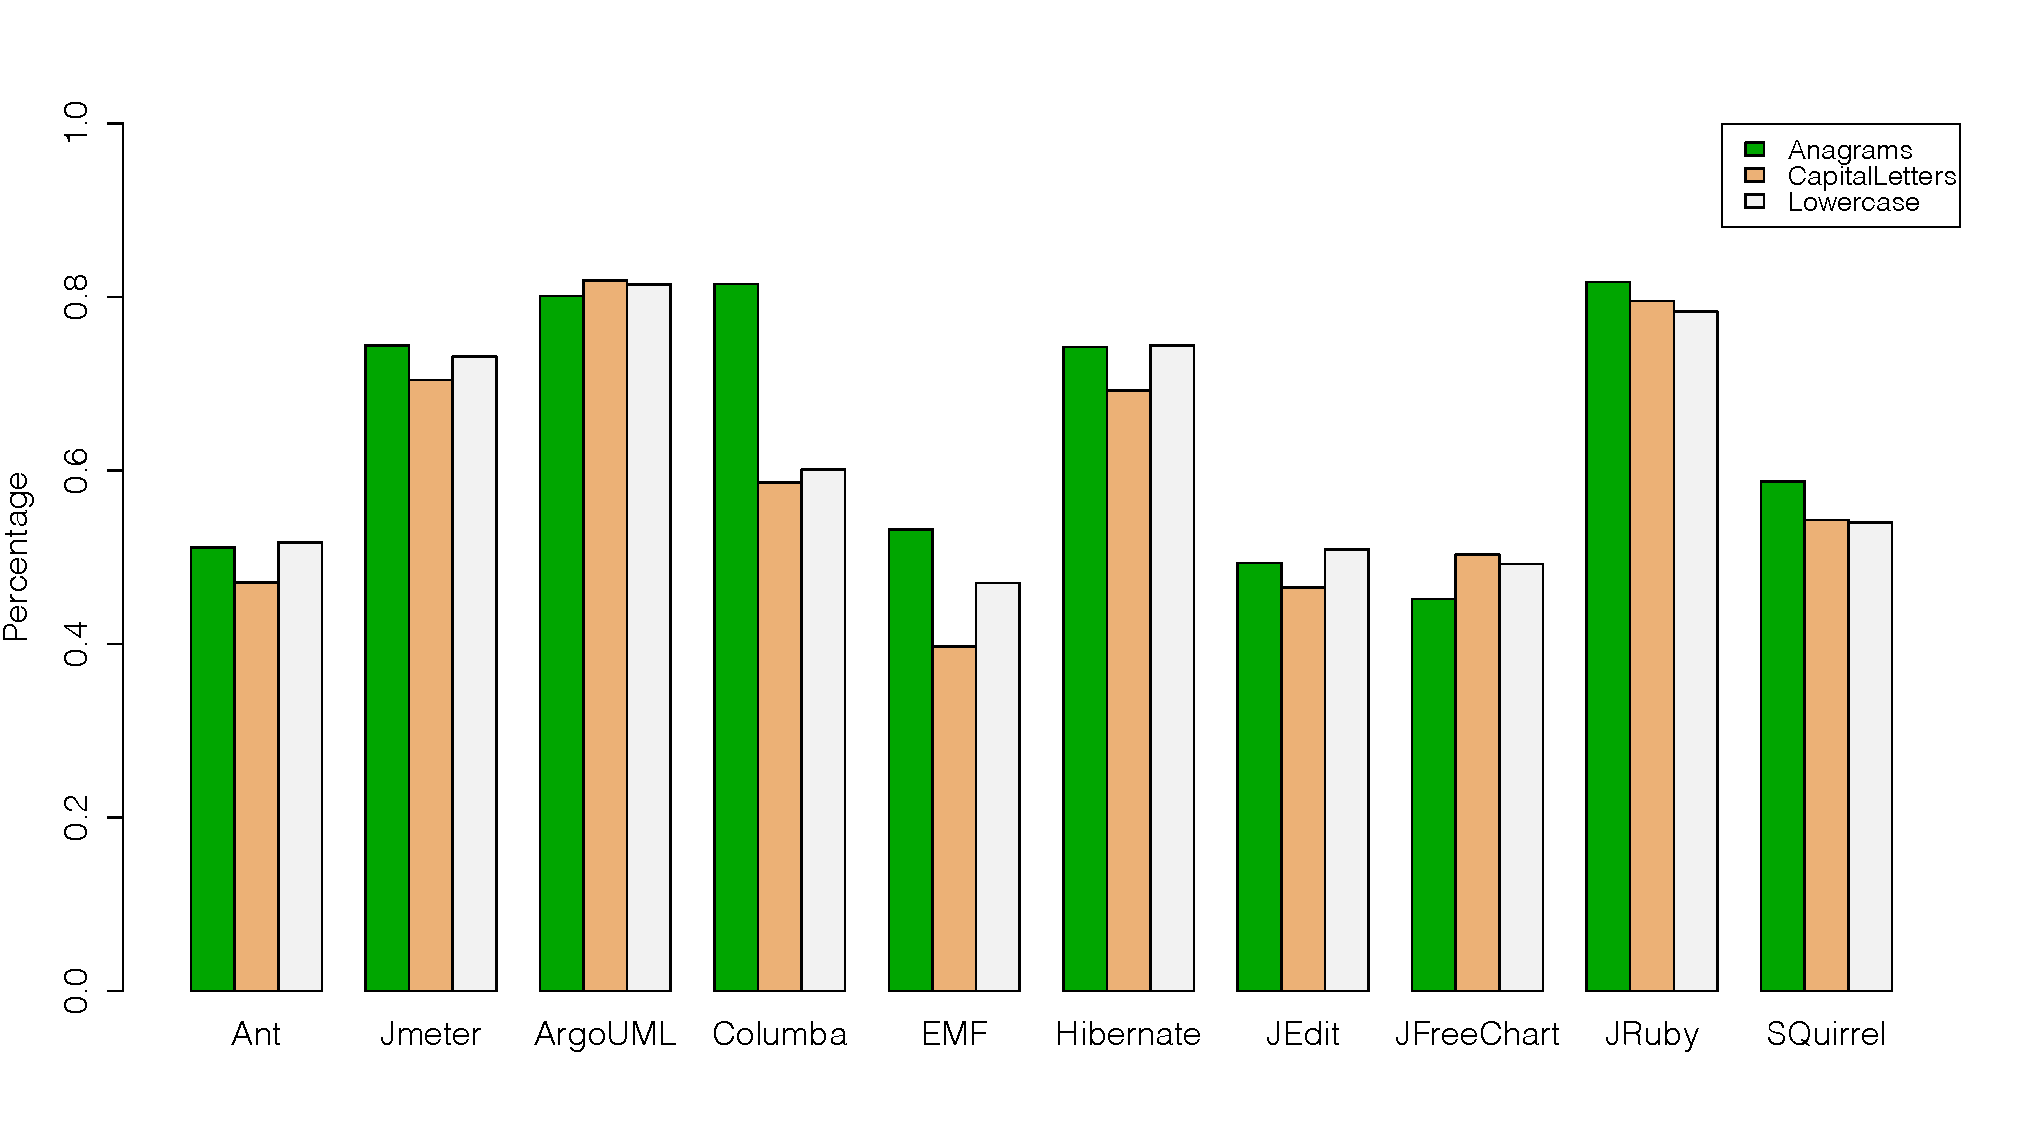
\includegraphics[width=0.50\textwidth]{figures/appendix/detailed_comparison_design_training_dataset.pdf}
  \vspace{-3mm}
  \caption{Detailed comparison of the changes in the design training datasets}
  \label{fig:detailed_comparison_design_training_dataset}
\end{figure}

\begin{figure}[thb!]
  \centering
  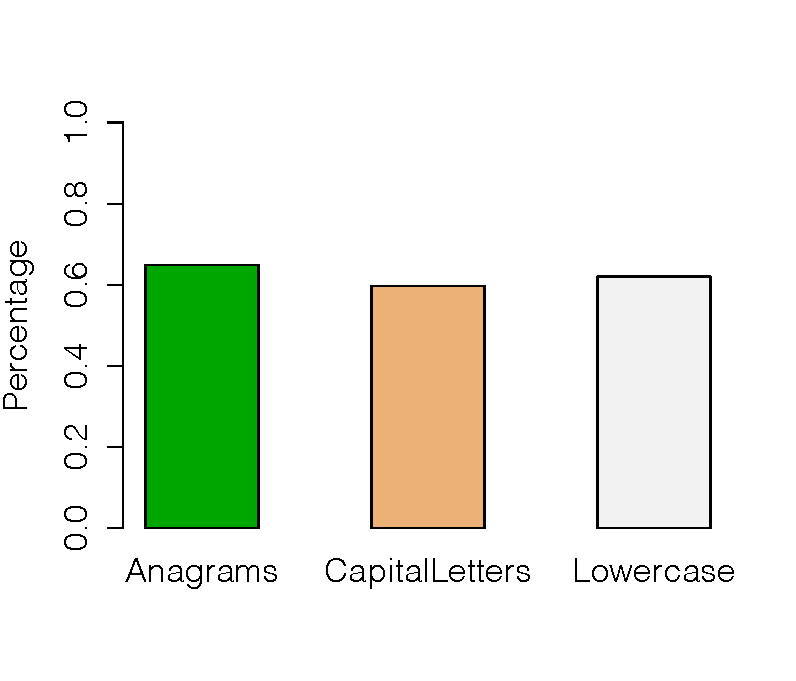
\includegraphics[width=0.50\textwidth]{figures/appendix/average_comparison_design_training_dataset.pdf}
  \vspace{-3mm}
  \caption{Average comparison of the changes in the design training datasets}
  \label{fig:average_comparison_design_training_dataset}
\end{figure}

\begin{table}[!hbt]
    \begin{center}
        \caption{Effects in the F1 measure of the Design training datasets}
        \label{tbl:detailed_comparison_design_training_dataset}
        \begin{tabular}{l| c c c}
        \toprule
        \thead{Project} & \thead{Anagrams\\Dataset} & \thead{Capitalized\\Dataset} & \thead{Lowercase\\Dataset}\\
        \midrule
        Apache Ant    &  0.511   & 0.471 &  0.517    \\
        Apache Jmeter &  0.744   & 0.704 &  0.731    \\
        ArgoUML       &  0.801   & 0.819 &  0.814    \\
        Columba       &  0.815   & 0.586 &  0.601    \\
        EMF           &  0.532   & 0.397 &  0.470    \\
        Hibernate     &  0.742   & 0.692 &  0.744    \\
        JEdit         &  0.493   & 0.465 &  0.509    \\
        JFreeChart    &  0.452   & 0.503 &  0.492    \\
        JRuby         &  0.817   & 0.795 &  0.783    \\
        SQuirrel      &  0.587   & 0.543 &  0.540    \\
        \bottomrule
        \end{tabular}
    \end{center}    
\end{table}

\clearpage

\begin{figure}[thb!]
  \centering
  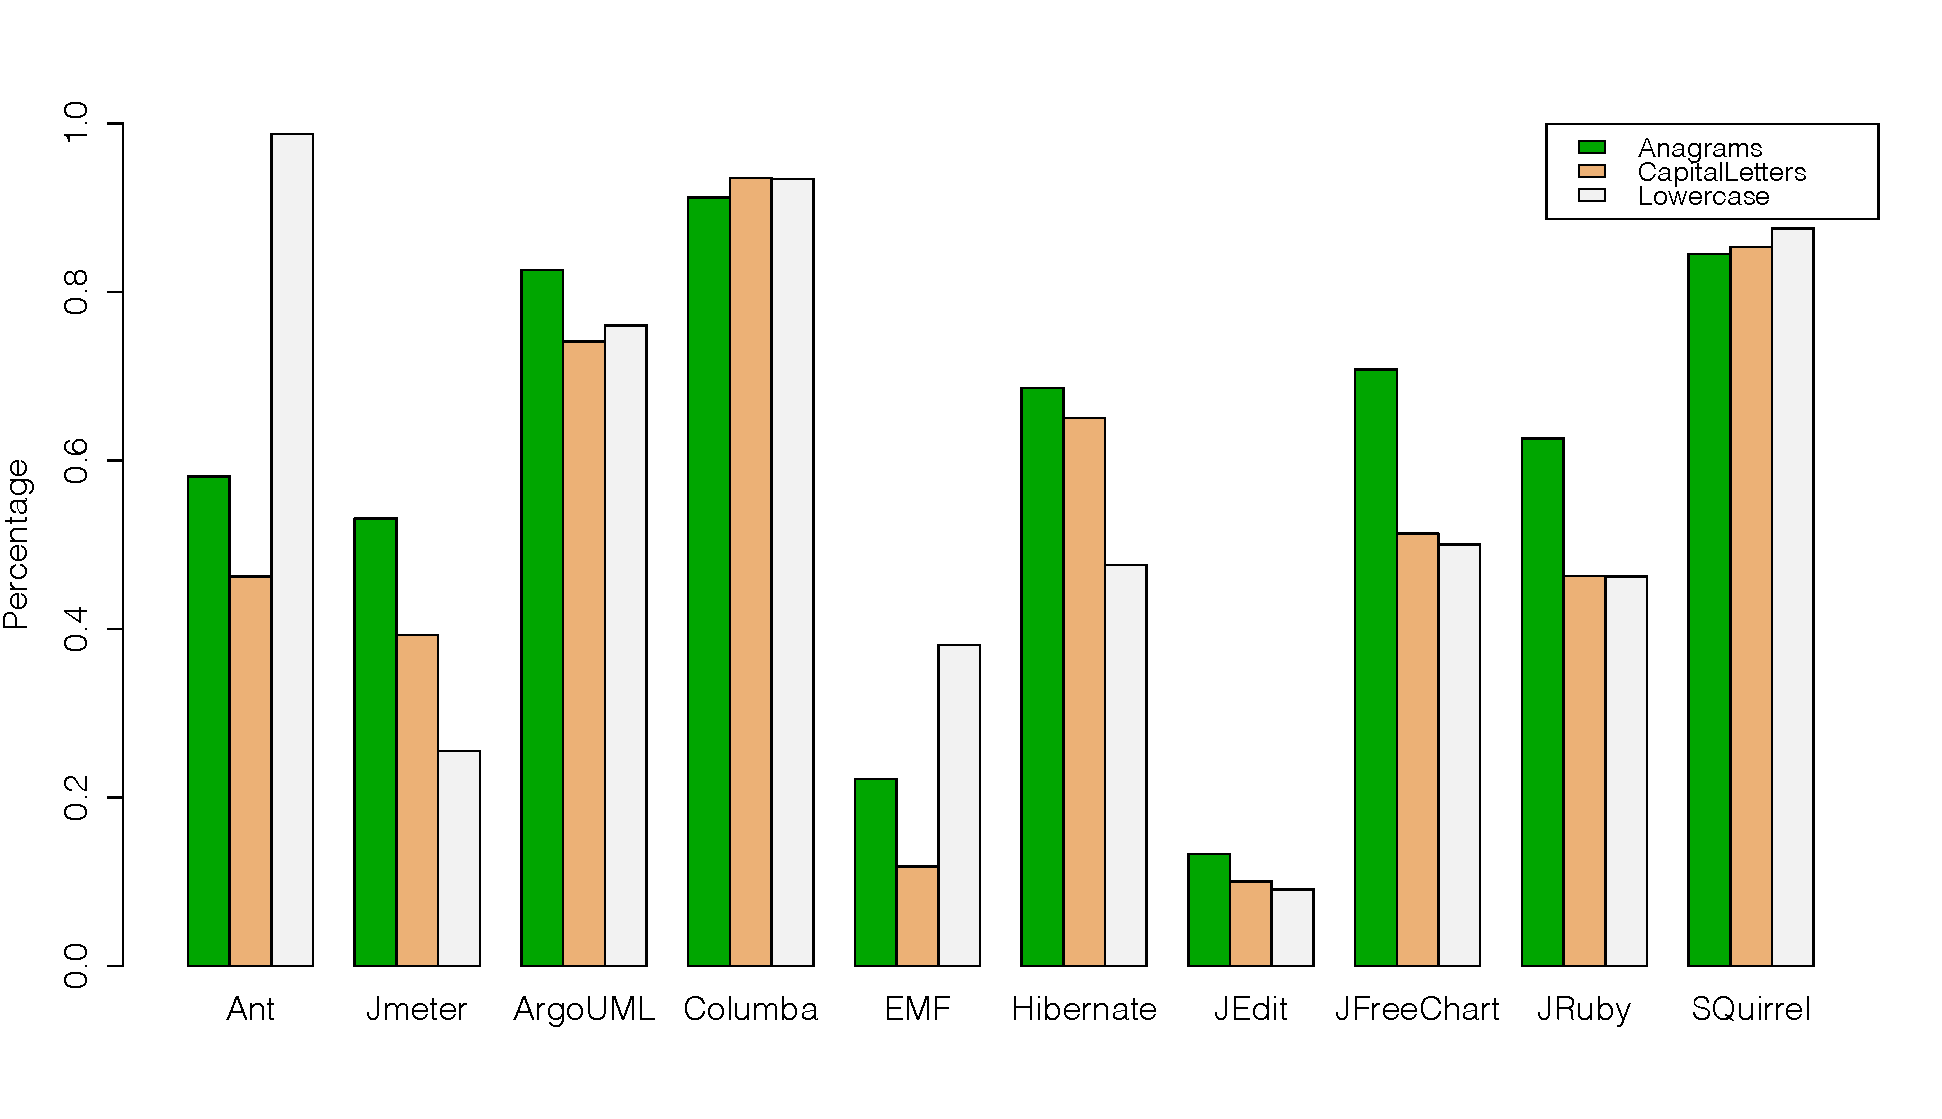
\includegraphics[width=0.50\textwidth]{figures/appendix/detailed_comparison_requirement_training_dataset.pdf}
  \vspace{-3mm}
  \caption{Detailed comparison of the changes in the requirements training datasets}
  \label{fig:detailed_comparison_requirement_training_dataset}
\end{figure}

\begin{figure}[thb!]
  \centering
  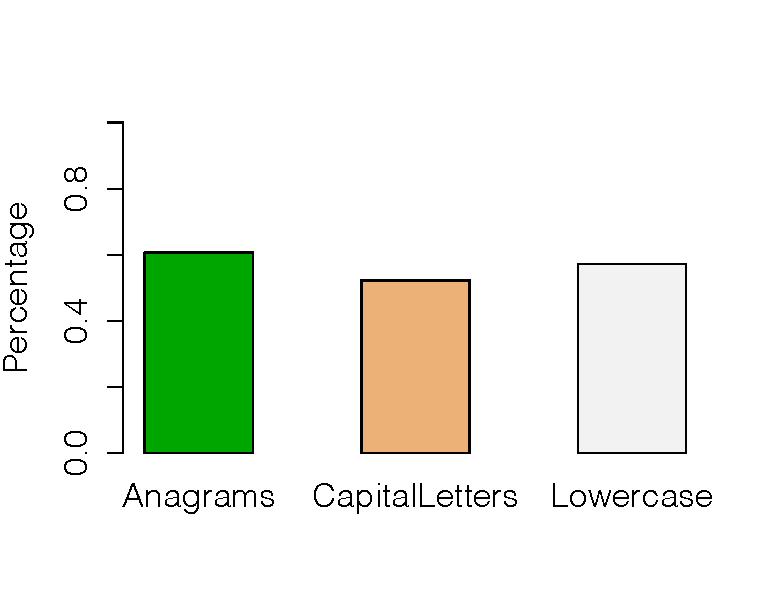
\includegraphics[width=0.50\textwidth]{figures/appendix/average_comparison_requeriment_training_dataset.pdf}
  \vspace{-3mm}
  \caption{Average comparison of the changes in the requirements training datasets}
  \label{fig:average_comparison_requirement_training_dataset}
\end{figure}

\begin{table}[!hbt]
    \begin{center}
        \caption{Effects in the F1 measure of the Requirements training datasets}
        \label{tbl:detailed_comparison_requirement_training_dataset}
        \begin{tabular}{l| c c c}
        \toprule
        \thead{Project} & \thead{Anagrams\\Dataset} & \thead{Capitalized\\Dataset} & \thead{Lowercase\\Dataset}\\
        \midrule
        Apache Ant    &  0.581 & 0.462 & 0.987  \\
        Apache Jmeter &  0.531 & 0.393 & 0.255  \\
        ArgoUML       &  0.826 & 0.741 & 0.760  \\
        Columba       &  0.912 & 0.935 & 0.934  \\
        EMF           &  0.222 & 0.118 & 0.381  \\
        Hibernate     &  0.686 & 0.650 & 0.476  \\
        JEdit         &  0.133 & 0.100 & 0.091  \\
        JFreeChart    &  0.708 & 0.513 & 0.500  \\
        JRuby         &  0.626 & 0.463 & 0.462  \\
        SQuirrel      &  0.845 & 0.853 & 0.875  \\
        \bottomrule
        \end{tabular}
    \end{center}    
\end{table}

